% Options for packages loaded elsewhere
\PassOptionsToPackage{unicode}{hyperref}
\PassOptionsToPackage{hyphens}{url}
\PassOptionsToPackage{dvipsnames,svgnames,x11names}{xcolor}
%
\documentclass[
]{article}
\usepackage{amsmath,amssymb}
\usepackage{lmodern}
\usepackage{iftex}
\ifPDFTeX
  \usepackage[T1]{fontenc}
  \usepackage[utf8]{inputenc}
  \usepackage{textcomp} % provide euro and other symbols
\else % if luatex or xetex
  \usepackage{unicode-math}
  \defaultfontfeatures{Scale=MatchLowercase}
  \defaultfontfeatures[\rmfamily]{Ligatures=TeX,Scale=1}
  \setmainfont[]{fouriernc}
\fi
% Use upquote if available, for straight quotes in verbatim environments
\IfFileExists{upquote.sty}{\usepackage{upquote}}{}
\IfFileExists{microtype.sty}{% use microtype if available
  \usepackage[]{microtype}
  \UseMicrotypeSet[protrusion]{basicmath} % disable protrusion for tt fonts
}{}
\makeatletter
\@ifundefined{KOMAClassName}{% if non-KOMA class
  \IfFileExists{parskip.sty}{%
    \usepackage{parskip}
  }{% else
    \setlength{\parindent}{0pt}
    \setlength{\parskip}{6pt plus 2pt minus 1pt}}
}{% if KOMA class
  \KOMAoptions{parskip=half}}
\makeatother
\usepackage{xcolor}
\usepackage[margin=1in]{geometry}
\usepackage{color}
\usepackage{fancyvrb}
\newcommand{\VerbBar}{|}
\newcommand{\VERB}{\Verb[commandchars=\\\{\}]}
\DefineVerbatimEnvironment{Highlighting}{Verbatim}{commandchars=\\\{\}}
% Add ',fontsize=\small' for more characters per line
\usepackage{framed}
\definecolor{shadecolor}{RGB}{248,248,248}
\newenvironment{Shaded}{\begin{snugshade}}{\end{snugshade}}
\newcommand{\AlertTok}[1]{\textcolor[rgb]{0.94,0.16,0.16}{#1}}
\newcommand{\AnnotationTok}[1]{\textcolor[rgb]{0.56,0.35,0.01}{\textbf{\textit{#1}}}}
\newcommand{\AttributeTok}[1]{\textcolor[rgb]{0.77,0.63,0.00}{#1}}
\newcommand{\BaseNTok}[1]{\textcolor[rgb]{0.00,0.00,0.81}{#1}}
\newcommand{\BuiltInTok}[1]{#1}
\newcommand{\CharTok}[1]{\textcolor[rgb]{0.31,0.60,0.02}{#1}}
\newcommand{\CommentTok}[1]{\textcolor[rgb]{0.56,0.35,0.01}{\textit{#1}}}
\newcommand{\CommentVarTok}[1]{\textcolor[rgb]{0.56,0.35,0.01}{\textbf{\textit{#1}}}}
\newcommand{\ConstantTok}[1]{\textcolor[rgb]{0.00,0.00,0.00}{#1}}
\newcommand{\ControlFlowTok}[1]{\textcolor[rgb]{0.13,0.29,0.53}{\textbf{#1}}}
\newcommand{\DataTypeTok}[1]{\textcolor[rgb]{0.13,0.29,0.53}{#1}}
\newcommand{\DecValTok}[1]{\textcolor[rgb]{0.00,0.00,0.81}{#1}}
\newcommand{\DocumentationTok}[1]{\textcolor[rgb]{0.56,0.35,0.01}{\textbf{\textit{#1}}}}
\newcommand{\ErrorTok}[1]{\textcolor[rgb]{0.64,0.00,0.00}{\textbf{#1}}}
\newcommand{\ExtensionTok}[1]{#1}
\newcommand{\FloatTok}[1]{\textcolor[rgb]{0.00,0.00,0.81}{#1}}
\newcommand{\FunctionTok}[1]{\textcolor[rgb]{0.00,0.00,0.00}{#1}}
\newcommand{\ImportTok}[1]{#1}
\newcommand{\InformationTok}[1]{\textcolor[rgb]{0.56,0.35,0.01}{\textbf{\textit{#1}}}}
\newcommand{\KeywordTok}[1]{\textcolor[rgb]{0.13,0.29,0.53}{\textbf{#1}}}
\newcommand{\NormalTok}[1]{#1}
\newcommand{\OperatorTok}[1]{\textcolor[rgb]{0.81,0.36,0.00}{\textbf{#1}}}
\newcommand{\OtherTok}[1]{\textcolor[rgb]{0.56,0.35,0.01}{#1}}
\newcommand{\PreprocessorTok}[1]{\textcolor[rgb]{0.56,0.35,0.01}{\textit{#1}}}
\newcommand{\RegionMarkerTok}[1]{#1}
\newcommand{\SpecialCharTok}[1]{\textcolor[rgb]{0.00,0.00,0.00}{#1}}
\newcommand{\SpecialStringTok}[1]{\textcolor[rgb]{0.31,0.60,0.02}{#1}}
\newcommand{\StringTok}[1]{\textcolor[rgb]{0.31,0.60,0.02}{#1}}
\newcommand{\VariableTok}[1]{\textcolor[rgb]{0.00,0.00,0.00}{#1}}
\newcommand{\VerbatimStringTok}[1]{\textcolor[rgb]{0.31,0.60,0.02}{#1}}
\newcommand{\WarningTok}[1]{\textcolor[rgb]{0.56,0.35,0.01}{\textbf{\textit{#1}}}}
\usepackage{graphicx}
\makeatletter
\def\maxwidth{\ifdim\Gin@nat@width>\linewidth\linewidth\else\Gin@nat@width\fi}
\def\maxheight{\ifdim\Gin@nat@height>\textheight\textheight\else\Gin@nat@height\fi}
\makeatother
% Scale images if necessary, so that they will not overflow the page
% margins by default, and it is still possible to overwrite the defaults
% using explicit options in \includegraphics[width, height, ...]{}
\setkeys{Gin}{width=\maxwidth,height=\maxheight,keepaspectratio}
% Set default figure placement to htbp
\makeatletter
\def\fps@figure{htbp}
\makeatother
\setlength{\emergencystretch}{3em} % prevent overfull lines
\providecommand{\tightlist}{%
  \setlength{\itemsep}{0pt}\setlength{\parskip}{0pt}}
\setcounter{secnumdepth}{-\maxdimen} % remove section numbering
\newlength{\cslhangindent}
\setlength{\cslhangindent}{1.5em}
\newlength{\csllabelwidth}
\setlength{\csllabelwidth}{3em}
\newlength{\cslentryspacingunit} % times entry-spacing
\setlength{\cslentryspacingunit}{\parskip}
\newenvironment{CSLReferences}[2] % #1 hanging-ident, #2 entry spacing
 {% don't indent paragraphs
  \setlength{\parindent}{0pt}
  % turn on hanging indent if param 1 is 1
  \ifodd #1
  \let\oldpar\par
  \def\par{\hangindent=\cslhangindent\oldpar}
  \fi
  % set entry spacing
  \setlength{\parskip}{#2\cslentryspacingunit}
 }%
 {}
\usepackage{calc}
\newcommand{\CSLBlock}[1]{#1\hfill\break}
\newcommand{\CSLLeftMargin}[1]{\parbox[t]{\csllabelwidth}{#1}}
\newcommand{\CSLRightInline}[1]{\parbox[t]{\linewidth - \csllabelwidth}{#1}\break}
\newcommand{\CSLIndent}[1]{\hspace{\cslhangindent}#1}
\newcommand{\indep}{\perp \!\!\! \perp}
\usepackage[T1]{fontenc}
\usepackage{fouriernc}
\usepackage{setspace}\onehalfspacing
\usepackage{amsfonts}
\usepackage{dcolumn}
\usepackage{pifont}
\usepackage{booktabs}
\usepackage{placeins}
\usepackage{booktabs}
\usepackage{longtable}
\usepackage{array}
\usepackage{multirow}
\usepackage{wrapfig}
\usepackage{float}
\usepackage{colortbl}
\usepackage{pdflscape}
\usepackage{tabu}
\usepackage{threeparttable}
\usepackage{threeparttablex}
\usepackage[normalem]{ulem}
\usepackage{makecell}
\usepackage{xcolor}
\usepackage{siunitx}

  \newcolumntype{d}{S[
    input-open-uncertainty=,
    input-close-uncertainty=,
    parse-numbers = false,
    table-align-text-pre=false,
    table-align-text-post=false
  ]}
  
\ifLuaTeX
  \usepackage{selnolig}  % disable illegal ligatures
\fi
\IfFileExists{bookmark.sty}{\usepackage{bookmark}}{\usepackage{hyperref}}
\IfFileExists{xurl.sty}{\usepackage{xurl}}{} % add URL line breaks if available
\urlstyle{same} % disable monospaced font for URLs
\hypersetup{
  pdftitle={Analysing Vote Choice Data},
  pdfauthor={Jacob Edenhofer},
  colorlinks=true,
  linkcolor={cyan},
  filecolor={Maroon},
  citecolor={Blue},
  urlcolor={magenta},
  pdfcreator={LaTeX via pandoc}}

\title{Analysing Vote Choice Data}
\usepackage{etoolbox}
\makeatletter
\providecommand{\subtitle}[1]{% add subtitle to \maketitle
  \apptocmd{\@title}{\par {\large #1 \par}}{}{}
}
\makeatother
\subtitle{Assignment 1}
\author{Jacob Edenhofer\footnote{\href{mailto:jacob.edenhofer@some.ox.ac.uk}{\nolinkurl{jacob.edenhofer@some.ox.ac.uk}}}}
\date{03 May 2023}

\begin{document}
\maketitle

\hypertarget{preliminaries}{%
\section{Preliminaries}\label{preliminaries}}

Let us start by importing the necessary packages and data. Please note:
I have included the questions in brown to indicate which (sub-)questions
a given answer belongs to.

\begin{Shaded}
\begin{Highlighting}[]
\CommentTok{\# packages}
\FunctionTok{library}\NormalTok{(tidyverse) }\CommentTok{\# ggplot, dplyr, }
\FunctionTok{library}\NormalTok{(modelsummary) }\CommentTok{\# summary statistics, regression tables}
\FunctionTok{library}\NormalTok{(janitor) }\CommentTok{\# data cleaning }
\FunctionTok{library}\NormalTok{(scales) }\CommentTok{\# add percentages, dates, etc. to plots }
\FunctionTok{library}\NormalTok{(haven) }\CommentTok{\# importing Stata data}
\FunctionTok{library}\NormalTok{(here) }\CommentTok{\# relative paths to ensure maximum replicability }
\FunctionTok{library}\NormalTok{(kableExtra) }\CommentTok{\# tables}
\FunctionTok{library}\NormalTok{(ggeffects) }\CommentTok{\# obtain and plot predicted values }
\FunctionTok{library}\NormalTok{(nnet) }\CommentTok{\# mulitnomial model}

\CommentTok{\# import data}
\NormalTok{ah21 }\OtherTok{\textless{}{-}} \FunctionTok{read\_dta}\NormalTok{(}\FunctionTok{paste0}\NormalTok{(}\FunctionTok{here}\NormalTok{(), }\StringTok{"/Data/ESS2018GER.dta"}\NormalTok{))}
\end{Highlighting}
\end{Shaded}

\hypertarget{exercise-1}{%
\section{Exercise 1}\label{exercise-1}}

\hypertarget{section}{%
\subsection{1.1}\label{section}}

\textcolor{brown}{(a) Get a sense of which variables and how many observations are present in the dataset, and make sure that all the variables are in the correct format: re-scale them when you find it appropriate. You may also want to use function `summary()` to get a sense of how many missing values (if any) are present and if some variables are more problematic than others.
(b) Compute the mean of relevant variables and report it in a table.
(c) Make sure that all the dichotomous variables are in a “viable” format (0 / 1).}

To answer these three questions, I will proceed in two steps:

\begin{itemize}
\item
  I will transform the two dummy variables, gender (\texttt{gndr}) and
  (non-)membership of an ethnic minority (\texttt{blgetmg}), into binary
  (0/1) format to answer part (c).

  \begin{itemize}
  \tightlist
  \item
    For the purposes of summarising the data, I will not rescale the
    variables.
  \end{itemize}
\item
  To answer part (b), I will use the \texttt{modelsummary} package's
  \texttt{datasummary\_skim()} function to summarise the
  data.\footnote{I prefer this function to the \texttt{summary()}
    function since it produces roughly the same output, but can be more
    easily used to produce summary tables via the \texttt{modelsummary}
    package.} In doing so, I will treat the ordered\footnote{For ordered
    categrocial variables, higher values correspond to greater/lower
    support for a given statement; increases in these variables
    therefore have substantively meaningful interpretations. This is not
    the case for non-ordered categorical variables, such as
    \texttt{prtvede1}, where the different values indicate different
    parties, rather than varying levels of support.} categorical
  variables (\texttt{ppltrst}, \texttt{gincdif}, \texttt{freehms},
  \texttt{imwbcnt}, \texttt{eduyrs}, \texttt{hinctnta}) as numeric
  variables, whereas I will treat the binary variables and the only
  non-ordered categorical variable (\texttt{prtvede1}) as factors.
\end{itemize}

Let us start with the dummy variables then:

\begin{Shaded}
\begin{Highlighting}[]
\NormalTok{ah21 }\OtherTok{\textless{}{-}}\NormalTok{ ah21 }\SpecialCharTok{\%\textgreater{}\%}
  \FunctionTok{mutate}\NormalTok{(}\AttributeTok{gndr1 =} \FunctionTok{ifelse}\NormalTok{(gndr }\SpecialCharTok{==} \DecValTok{1}\NormalTok{, }\DecValTok{1}\NormalTok{, }\DecValTok{0}\NormalTok{), }\CommentTok{\# 1 for male, 0 for female}
         \AttributeTok{blgetmg1 =} \FunctionTok{ifelse}\NormalTok{(blgetmg }\SpecialCharTok{==} \DecValTok{1}\NormalTok{, }\DecValTok{1}\NormalTok{, }\DecValTok{0}\NormalTok{)) }\CommentTok{\# 1 for ethnic minority, 0 for not }
\end{Highlighting}
\end{Shaded}

Next, I will compute the mean for all non-ordered categorical variables
(and other relevant summary statistics) via the following piece of
code.\footnote{As can be gleaned from the
  \href{https://ess-search.nsd.no/en/study/bdc7c350-1029-4cb3-9d5e-53f668b8fa74}{ESS
  codebook} for round nine, higher values of \texttt{ppltrst} (first
  row) indicate greater levels of trust. In contrast, higher values of
  \texttt{gincdif} indicate less support for redistribution (second
  row). Similarly, lower values of \texttt{freehms} indicate less
  support for the LGBT+ people's right to live as they wish. Higher
  values of \texttt{imwbcnt} indicate greater agreement with the view
  that immigrants make the country a better place to live (third row).}
For emphasis, I have coloured the relevant column in dark blue. It is
also worth noting that I have set the \texttt{histogram} argument to
\texttt{FALSE} since the resulting histograms are distracting - they are
too small to read and not labelled.\footnote{See the appendix for a
  version of this table that includes histograms.}

\begin{Shaded}
\begin{Highlighting}[]
\NormalTok{ah21 }\SpecialCharTok{\%\textgreater{}\%}
  \FunctionTok{select}\NormalTok{(}\SpecialCharTok{{-}}\FunctionTok{c}\NormalTok{(cntry, }\FunctionTok{grep}\NormalTok{(}\StringTok{"gndr"}\NormalTok{, }\FunctionTok{names}\NormalTok{(.)), }\FunctionTok{grep}\NormalTok{(}\StringTok{"blgetmg"}\NormalTok{, }\FunctionTok{names}\NormalTok{(.)), prtvede1)) }\SpecialCharTok{\%\textgreater{}\%}
  \FunctionTok{datasummary\_skim}\NormalTok{(}\AttributeTok{output =} \StringTok{"kableExtra"}\NormalTok{, }\AttributeTok{histogram =}\NormalTok{ F,}
                   \AttributeTok{title =} \StringTok{"Summary statistics for ordered catgeorical variables"}\NormalTok{) }\SpecialCharTok{\%\textgreater{}\%}
  \FunctionTok{kable\_styling}\NormalTok{(}\AttributeTok{latex\_options =} \FunctionTok{c}\NormalTok{(}\StringTok{"scale\_down"}\NormalTok{, }\StringTok{"hold\_position"}\NormalTok{)) }\SpecialCharTok{\%\textgreater{}\%}
  \FunctionTok{column\_spec}\NormalTok{(}\DecValTok{4}\NormalTok{, }\AttributeTok{background =} \StringTok{"\#1F263C"}\NormalTok{, }\AttributeTok{color =} \StringTok{"white"}\NormalTok{) }\SpecialCharTok{\%\textgreater{}\%}
  \FunctionTok{add\_footnote}\NormalTok{(}\AttributeTok{label =} \StringTok{"Source: ESS round 9 (2018)"}\NormalTok{, }
               \AttributeTok{notation =} \StringTok{"none"}\NormalTok{) }
\end{Highlighting}
\end{Shaded}

\begin{table}[!h]

\caption{\label{tab:eda-ah21}Summary statistics for ordered catgeorical variables}
\centering
\resizebox{\linewidth}{!}{
\begin{tabular}[t]{lrr>{}rrrrr}
\toprule
  & Unique (\#) & Missing (\%) & Mean & SD & Min & Median & Max\\
\midrule
Most people can be trusted or you can't be too careful & 11 & 0 & \cellcolor[HTML]{1F263C}{\textcolor{white}{\num{5.6}}} & \num{2.2} & \num{0.0} & \num{6.0} & \num{10.0}\\
Government should reduce differences in income levels & 6 & 0 & \cellcolor[HTML]{1F263C}{\textcolor{white}{\num{2.1}}} & \num{1.0} & \num{1.0} & \num{2.0} & \num{5.0}\\
Gays and lesbians free to live life as they wish & 6 & 0 & \cellcolor[HTML]{1F263C}{\textcolor{white}{\num{1.7}}} & \num{0.8} & \num{1.0} & \num{2.0} & \num{5.0}\\
Immigrants make country worse or better place to live & 12 & 1 & \cellcolor[HTML]{1F263C}{\textcolor{white}{\num{5.4}}} & \num{2.2} & \num{0.0} & \num{5.0} & \num{10.0}\\
Years of full-time education completed & 25 & 0 & \cellcolor[HTML]{1F263C}{\textcolor{white}{\num{14.8}}} & \num{3.4} & \num{5.0} & \num{14.0} & \num{30.0}\\
Household's total net income, all sources & 11 & 8 & \cellcolor[HTML]{1F263C}{\textcolor{white}{\num{6.4}}} & \num{2.7} & \num{1.0} & \num{7.0} & \num{10.0}\\
\bottomrule
\multicolumn{8}{l}{\textsuperscript{} Source: ESS round 9 (2018)}\\
\end{tabular}}
\end{table}

Apart from the the usual summary statistics (mean, median, standard
deviation, minimum and maximum), the table also shows that there is one
variable in particular, \texttt{hinctnta}, for which there are
significant missing values (116 to be precise).\footnote{This number is
  obtained by running \texttt{sum(is.na(ah21\$hinctnta))}.} As a result,
some care must be exercised when using the income variable in
regressions since item non-response may be correlated with other
characteristics that also affect the dependent variable of interest
(i.e.~confounders).

For the non-ordered categorical variables, I modify the \texttt{type}
argument, yielding a table with columns indicating the number of
observations per category - both in raw terms and as a share of the
total number of observations. Hence, I run:

\begin{Shaded}
\begin{Highlighting}[]
\NormalTok{ah21 }\SpecialCharTok{\%\textgreater{}\%}
  \FunctionTok{select}\NormalTok{(}\StringTok{"Gender"} \OtherTok{=}\NormalTok{ gndr1, }\StringTok{"Member of ethnic minority"} \OtherTok{=}\NormalTok{ blgetmg1, }
         \StringTok{"Party voted for in last national election, Germany"} \OtherTok{=}\NormalTok{ prtvede1) }\SpecialCharTok{\%\textgreater{}\%}
  \CommentTok{\# factorise selected variables, and rename levels for readability }
  \FunctionTok{mutate}\NormalTok{(}\AttributeTok{Gender =} \FunctionTok{factor}\NormalTok{(Gender, }\AttributeTok{levels =} \FunctionTok{c}\NormalTok{(}\StringTok{"0"}\NormalTok{, }\StringTok{"1"}\NormalTok{), }
                         \CommentTok{\# see code above }
                         \AttributeTok{labels =} \FunctionTok{c}\NormalTok{(}\StringTok{"Female"}\NormalTok{, }\StringTok{"Male"}\NormalTok{)),}
         \StringTok{\textasciigrave{}}\AttributeTok{Member of ethnic minority}\StringTok{\textasciigrave{}} \OtherTok{=} \FunctionTok{factor}\NormalTok{(}\StringTok{\textasciigrave{}}\AttributeTok{Member of ethnic minority}\StringTok{\textasciigrave{}}\NormalTok{, }
                                              \AttributeTok{levels =} \FunctionTok{c}\NormalTok{(}\StringTok{"0"}\NormalTok{, }\StringTok{"1"}\NormalTok{), }
                                              \AttributeTok{labels =} \FunctionTok{c}\NormalTok{(}\StringTok{"No"}\NormalTok{, }\StringTok{"Yes"}\NormalTok{)),}
         \StringTok{\textasciigrave{}}\AttributeTok{Party voted for in last national election, Germany}\StringTok{\textasciigrave{}} \OtherTok{=} 
           \FunctionTok{factor}\NormalTok{(}\StringTok{\textasciigrave{}}\AttributeTok{Party voted for in last national election, Germany}\StringTok{\textasciigrave{}}\NormalTok{, }
                  \AttributeTok{levels =} \FunctionTok{c}\NormalTok{(}\StringTok{"1"}\NormalTok{, }\StringTok{"2"}\NormalTok{, }\StringTok{"3"}\NormalTok{, }\StringTok{"4"}\NormalTok{, }\StringTok{"5"}\NormalTok{, }\StringTok{"6"}\NormalTok{, }\StringTok{"7"}\NormalTok{, }\StringTok{"8"}\NormalTok{),}
                  \AttributeTok{labels =} \FunctionTok{c}\NormalTok{(}\StringTok{"CDU/CSU"}\NormalTok{, }\StringTok{"SPD"}\NormalTok{, }\StringTok{"LINKE"}\NormalTok{, }\StringTok{"Greens"}\NormalTok{, }\StringTok{"FDP"}\NormalTok{, }
                             \StringTok{"AfD"}\NormalTok{, }\StringTok{"Pirates"}\NormalTok{, }\StringTok{"NPD"}\NormalTok{))) }\SpecialCharTok{\%\textgreater{}\%}
  \FunctionTok{datasummary\_skim}\NormalTok{(}\AttributeTok{type =} \StringTok{"categorical"}\NormalTok{,}
                   \AttributeTok{output =} \StringTok{"kableExtra"}\NormalTok{, }
                   \AttributeTok{title =} \StringTok{"Summary statistics for non{-}ordered categorical variables"}\NormalTok{) }\SpecialCharTok{\%\textgreater{}\%}
  \FunctionTok{kable\_styling}\NormalTok{(}\AttributeTok{full\_width =}\NormalTok{ T, }\AttributeTok{latex\_options =} \StringTok{"hold\_position"}\NormalTok{) }\SpecialCharTok{\%\textgreater{}\%}
  \FunctionTok{column\_spec}\NormalTok{(}\DecValTok{1}\NormalTok{, }\AttributeTok{width =} \StringTok{"8cm"}\NormalTok{) }\SpecialCharTok{\%\textgreater{}\%}
  \FunctionTok{add\_footnote}\NormalTok{(}\AttributeTok{label =} \StringTok{"Round 9 of the ESS was run in 2018; \textquotesingle{}last national election\textquotesingle{} therefore refers to the 2017 German general election."}\NormalTok{, }
               \AttributeTok{notation =} \StringTok{"none"}\NormalTok{)}
\end{Highlighting}
\end{Shaded}

\begin{table}[!h]

\caption{\label{tab:ed-ah21-categorical}Summary statistics for non-ordered categorical variables}
\centering
\begin{tabu} to \linewidth {>{\raggedright\arraybackslash}p{8cm}>{\raggedright}X>{\raggedleft}X>{\raggedleft}X}
\toprule
  &    & N & \%\\
\midrule
Gender & Female & 731 & \num{47.7}\\
 & Male & 800 & \num{52.3}\\
Member of ethnic minority & No & 1471 & \num{96.1}\\
 & Yes & 57 & \num{3.7}\\
Party voted for in last national election, Germany & CDU/CSU & 606 & \num{39.6}\\
 & SPD & 400 & \num{26.1}\\
 & LINKE & 107 & \num{7.0}\\
 & Greens & 223 & \num{14.6}\\
 & FDP & 97 & \num{6.3}\\
 & AfD & 96 & \num{6.3}\\
 & Pirates & 1 & \num{0.1}\\
 & NPD & 1 & \num{0.1}\\
\bottomrule
\multicolumn{4}{l}{\textsuperscript{} Round 9 of the ESS was run in 2018; 'last national election' therefore refers to the}\\
\multicolumn{4}{l}{2017 German general election.}\\
\end{tabu}
\end{table}

Table 2 shows that:

\begin{itemize}
\tightlist
\item
  there are slightly more male respondents than female ones,
\item
  only 3.7\% of respondents are members of ethnic minorities, and
\item
  the vote share variables correspond only loosely\footnote{According to
    the
    \href{https://www.bundeswahlleiter.de/bundestagswahlen/2017/ergebnisse.html}{Bundeswahlleiter},
    the share of party votes (``Zweitstimmenanteile'') obtained by the
    respective parties in 2017 were: 32.9\% for the CDU/CSU, 20.5\% for
    the SPD, 12.6\% for the AfD, 10.7\% for the FDP, 9.2\% for the
    LINKE, and 8.9\% for the Greens. The NDP remained well below the
    five-percent threshold.} to the ones actually obtained by the
  respective parties in the 2017 national election, the last election
  before round nine of the ESS in 2018
\end{itemize}

\textcolor{brown}{(d) Represent the distribution of the variable measuring respondents’ years of formal education. Label the axes, pick a title, and add a solid, blue line at the median value and a red, dashed line at the mean value.}

To answer this question, I run the following code. For the purpose of
achieving maximum visual interpretability, I set the \texttt{binwidth}
argument to two, while the vertical lines are created via the
\texttt{geom\_vline()} functions. The warning messages indicate that
there is one missing value for \texttt{eduyrs}, entailing that the
histogram is based on 1530 observations.

\begin{Shaded}
\begin{Highlighting}[]
\NormalTok{ah21 }\SpecialCharTok{\%\textgreater{}\%}
  \FunctionTok{ggplot}\NormalTok{(}\FunctionTok{aes}\NormalTok{(}\AttributeTok{x =}\NormalTok{ eduyrs)) }\SpecialCharTok{+}
  \FunctionTok{geom\_histogram}\NormalTok{(}\FunctionTok{aes}\NormalTok{(}\AttributeTok{y =} \FunctionTok{after\_stat}\NormalTok{(density)), }\AttributeTok{binwidth =} \DecValTok{2}\NormalTok{, }\AttributeTok{colour =} \StringTok{"white"}\NormalTok{) }\SpecialCharTok{+}
  \FunctionTok{geom\_density}\NormalTok{(}\AttributeTok{linewidth =} \DecValTok{1}\NormalTok{) }\SpecialCharTok{+}
  \FunctionTok{geom\_vline}\NormalTok{(}\FunctionTok{aes}\NormalTok{(}\AttributeTok{xintercept =} \FunctionTok{mean}\NormalTok{(eduyrs, }\AttributeTok{na.rm =}\NormalTok{ T)), }
             \AttributeTok{colour =} \StringTok{"red"}\NormalTok{, }\AttributeTok{linetype =} \StringTok{"dashed"}\NormalTok{, }\AttributeTok{linewidth =} \DecValTok{1}\NormalTok{) }\SpecialCharTok{+}
  \FunctionTok{geom\_vline}\NormalTok{(}\FunctionTok{aes}\NormalTok{(}\AttributeTok{xintercept =} \FunctionTok{median}\NormalTok{(eduyrs)), }
             \AttributeTok{colour =} \StringTok{"blue"}\NormalTok{, }\AttributeTok{linewidth =} \DecValTok{1}\NormalTok{) }\SpecialCharTok{+}
  \FunctionTok{scale\_x\_continuous}\NormalTok{(}\StringTok{"Years of full{-}time education completed"}\NormalTok{, }\AttributeTok{breaks =} \FunctionTok{seq}\NormalTok{(}\DecValTok{5}\NormalTok{, }\DecValTok{30}\NormalTok{, }\DecValTok{5}\NormalTok{)) }\SpecialCharTok{+}
  \FunctionTok{expand\_limits}\NormalTok{(}\AttributeTok{y =} \FloatTok{0.15}\NormalTok{) }\SpecialCharTok{+}
  \FunctionTok{labs}\NormalTok{(}\AttributeTok{y =} \StringTok{"Density"}\NormalTok{, }\AttributeTok{title =} \StringTok{"Histogram of \textquotesingle{}years of full{-}time education completed\textquotesingle{}"}\NormalTok{, }
       \AttributeTok{caption =} \StringTok{"The red dashed line indicates the mean value, while the blue solid line indicates the median."}\NormalTok{) }\SpecialCharTok{+}
  \FunctionTok{theme\_bw}\NormalTok{() }
\end{Highlighting}
\end{Shaded}

\begin{verbatim}
## Warning: Removed 1 rows containing non-finite values (`stat_bin()`).
\end{verbatim}

\begin{verbatim}
## Warning: Removed 1 rows containing non-finite values (`stat_density()`).
\end{verbatim}

\begin{center}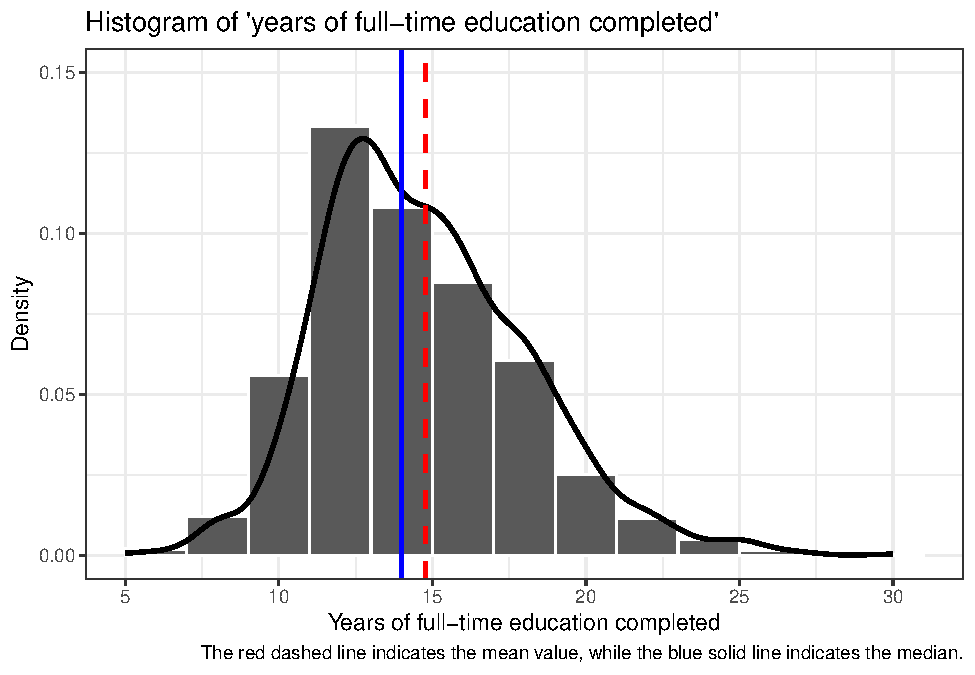
\includegraphics{AVCD-Assignment1-Edenhofer_files/figure-latex/distribution-eduyears-1} \end{center}

\textcolor{brown}{What do we learn about the distribution by looking at the mean and the median?}

As can be gleaned from the histogram, the mean value (14.8, see table 1)
exceeds the median (14, see table 1), implying that the distribution is
slightly skewed to the left, though the distribution of \texttt{eduyrs}
is close to what the theoretical normal distribution with mean 14.8 and
a standard deviation of 3.4 (see table 1) would look like.\footnote{The
  appendix contains a modified version of this figure, which includes
  the density line of this theoretical normal distribution. The latter
  is useful for detecting the slight left skew of the actual density
  line.}

\hypertarget{section-1}{%
\subsection{1.2}\label{section-1}}

I start by creating the dependent variables of interest by, first,
filtering out all those parties\footnote{Specifically,
  \texttt{ah21\_mod} excludes Die LINKE, the NPD, FDP and Pirates.} that
are not contained in table one of the online appendix
(\protect\hyperlink{ref-abou-chadi_brahmin_2021}{Abou-Chadi and Hix
2021}) and then dichotomising the remaining four levels:

\begin{Shaded}
\begin{Highlighting}[]
\NormalTok{ah21\_mod }\OtherTok{\textless{}{-}}\NormalTok{ ah21 }\SpecialCharTok{\%\textgreater{}\%}
  \FunctionTok{filter}\NormalTok{(}\SpecialCharTok{!}\NormalTok{prtvede1 }\SpecialCharTok{\%in\%} \FunctionTok{c}\NormalTok{(}\DecValTok{3}\NormalTok{, }\DecValTok{5}\NormalTok{, }\DecValTok{7}\NormalTok{, }\DecValTok{8}\NormalTok{)) }\SpecialCharTok{\%\textgreater{}\%}
  \FunctionTok{mutate}\NormalTok{(}\AttributeTok{piketty\_dv =} \FunctionTok{ifelse}\NormalTok{(prtvede1 }\SpecialCharTok{\%in\%} \FunctionTok{c}\NormalTok{(}\DecValTok{2}\NormalTok{, }\DecValTok{4}\NormalTok{), }\DecValTok{1}\NormalTok{, }\DecValTok{0}\NormalTok{)) }\CommentTok{\# left equals 1, right equals zero }
\end{Highlighting}
\end{Shaded}

\textcolor{brown}{(a) Does the distribution of years of education vary between those voting left and those who do not? For simplicity reasons, group years of education in four possible classes (Hint: use the dummy variable `a la Piketty).}

I will, first, create a four-part education variable and, then, plot the
distribution of education groups by left-right vote choice. The range of
\texttt{eduyrs} is, as table 1 shows, \([5, 30]\). I partition this
interval into the following four groups:

\begin{itemize}
\tightlist
\item
  \([5, 10)\) corresponds roughly to less than GCSE
\item
  \([10, 15)\) corresponds roughly to A-levels and university drop-outs
\item
  \([15, 20)\) corresponds roughly to university graduates
\item
  \([20, 30]\) corresponds roughly to those with post-graduate
  qualifications
\end{itemize}

\begin{Shaded}
\begin{Highlighting}[]
\CommentTok{\# education variable }
\NormalTok{ah21\_mod }\OtherTok{\textless{}{-}}\NormalTok{ ah21\_mod }\SpecialCharTok{\%\textgreater{}\%}
  \FunctionTok{mutate}\NormalTok{(}\AttributeTok{ed\_4part =} \FunctionTok{case\_when}\NormalTok{((eduyrs }\SpecialCharTok{\textgreater{}=} \DecValTok{5} \SpecialCharTok{\&}\NormalTok{ eduyrs }\SpecialCharTok{\textless{}} \DecValTok{10}\NormalTok{) }\SpecialCharTok{\textasciitilde{}} \StringTok{"[5, 10)"}\NormalTok{,}
\NormalTok{                              (eduyrs }\SpecialCharTok{\textgreater{}=} \DecValTok{10} \SpecialCharTok{\&}\NormalTok{ eduyrs }\SpecialCharTok{\textless{}} \DecValTok{15}\NormalTok{) }\SpecialCharTok{\textasciitilde{}} \StringTok{"[10, 15)"}\NormalTok{,}
\NormalTok{                              (eduyrs }\SpecialCharTok{\textgreater{}=} \DecValTok{15} \SpecialCharTok{\&}\NormalTok{ eduyrs }\SpecialCharTok{\textless{}} \DecValTok{20}\NormalTok{) }\SpecialCharTok{\textasciitilde{}} \StringTok{"[15, 20)"}\NormalTok{, }
\NormalTok{                              (eduyrs }\SpecialCharTok{\textgreater{}=} \DecValTok{20} \SpecialCharTok{\&}\NormalTok{ eduyrs }\SpecialCharTok{\textless{}=} \DecValTok{30}\NormalTok{) }\SpecialCharTok{\textasciitilde{}} \StringTok{"[20, 30]"}\NormalTok{))}
\CommentTok{\# plot }
\NormalTok{ah21\_mod }\SpecialCharTok{\%\textgreater{}\%}
  \CommentTok{\# omit missing observation to avoid cluttered plot }
  \FunctionTok{filter}\NormalTok{(}\SpecialCharTok{!}\FunctionTok{is.na}\NormalTok{(eduyrs)) }\SpecialCharTok{\%\textgreater{}\%}
  \CommentTok{\# compute shares in each education group by vote choice }
  \FunctionTok{count}\NormalTok{(}\FunctionTok{factor}\NormalTok{(piketty\_dv), ed\_4part) }\SpecialCharTok{\%\textgreater{}\%}
  \FunctionTok{rename}\NormalTok{(}\StringTok{"piketty"} \OtherTok{=} \StringTok{\textasciigrave{}}\AttributeTok{factor(piketty\_dv)}\StringTok{\textasciigrave{}}\NormalTok{) }\SpecialCharTok{\%\textgreater{}\%} \CommentTok{\# rename for convenience }
  \FunctionTok{group\_by}\NormalTok{(piketty) }\SpecialCharTok{\%\textgreater{}\%}
  \FunctionTok{mutate}\NormalTok{(}\AttributeTok{share =} \FunctionTok{round}\NormalTok{(}\DecValTok{100}\SpecialCharTok{*}\NormalTok{(n}\SpecialCharTok{/}\FunctionTok{sum}\NormalTok{(n)), }\DecValTok{1}\NormalTok{)) }\SpecialCharTok{\%\textgreater{}\%}
  \CommentTok{\# plot this data frame }
  \FunctionTok{ggplot}\NormalTok{(}\FunctionTok{aes}\NormalTok{(}\AttributeTok{x =}\NormalTok{ piketty, }\AttributeTok{y =}\NormalTok{ share, }
             \AttributeTok{fill =} \FunctionTok{factor}\NormalTok{(ed\_4part, }
                           \AttributeTok{levels =} \FunctionTok{c}\NormalTok{(}\StringTok{"[5, 10)"}\NormalTok{, }\StringTok{"[10, 15)"}\NormalTok{, }
                                      \StringTok{"[15, 20)"}\NormalTok{, }\StringTok{"[20, 30]"}\NormalTok{)))) }\SpecialCharTok{+}
  \FunctionTok{geom\_col}\NormalTok{(}\AttributeTok{position =} \StringTok{"dodge"}\NormalTok{) }\SpecialCharTok{+}
  \FunctionTok{geom\_text}\NormalTok{(}\FunctionTok{aes}\NormalTok{(}\AttributeTok{label =}\NormalTok{ share), }
            \AttributeTok{position =} \FunctionTok{position\_dodge}\NormalTok{(}\AttributeTok{width =} \FloatTok{0.9}\NormalTok{),}
            \AttributeTok{vjust =} \SpecialCharTok{{-}}\FloatTok{0.2}\NormalTok{) }\SpecialCharTok{+}
  \FunctionTok{scale\_fill\_viridis\_d}\NormalTok{(}\StringTok{"Education in years"}\NormalTok{, }\AttributeTok{direction =} \SpecialCharTok{{-}}\DecValTok{1}\NormalTok{) }\SpecialCharTok{+}
  \FunctionTok{scale\_y\_continuous}\NormalTok{(}\StringTok{"Share of respondents"}\NormalTok{,}
                     \AttributeTok{breaks =} \FunctionTok{seq}\NormalTok{(}\DecValTok{0}\NormalTok{, }\DecValTok{60}\NormalTok{, }\DecValTok{15}\NormalTok{),}
                     \AttributeTok{labels =} \FunctionTok{label\_percent}\NormalTok{(}\AttributeTok{scale =} \DecValTok{1}\NormalTok{)) }\SpecialCharTok{+}
  \FunctionTok{scale\_x\_discrete}\NormalTok{(}\StringTok{"Party bloc voted for in last national election"}\NormalTok{, }
                   \AttributeTok{labels =} \FunctionTok{c}\NormalTok{(}\StringTok{"0"} \OtherTok{=} \StringTok{"Right"}\NormalTok{, }
                              \StringTok{"1"} \OtherTok{=} \StringTok{"Left"}\NormalTok{)) }\SpecialCharTok{+}
  \FunctionTok{expand\_limits}\NormalTok{(}\AttributeTok{y =} \DecValTok{60}\NormalTok{) }\SpecialCharTok{+}
  \FunctionTok{labs}\NormalTok{(}\AttributeTok{x =} \StringTok{"Education in years"}\NormalTok{, }\AttributeTok{y =} \StringTok{"Share of respondent"}\NormalTok{,}
       \AttributeTok{title =} \StringTok{"Distribution of education by dichotomous vote choice"}\NormalTok{) }\SpecialCharTok{+}
  \FunctionTok{theme\_bw}\NormalTok{() }\SpecialCharTok{+}
  \FunctionTok{theme}\NormalTok{(}\AttributeTok{legend.position =} \StringTok{"bottom"}\NormalTok{)}
\end{Highlighting}
\end{Shaded}

\begin{center}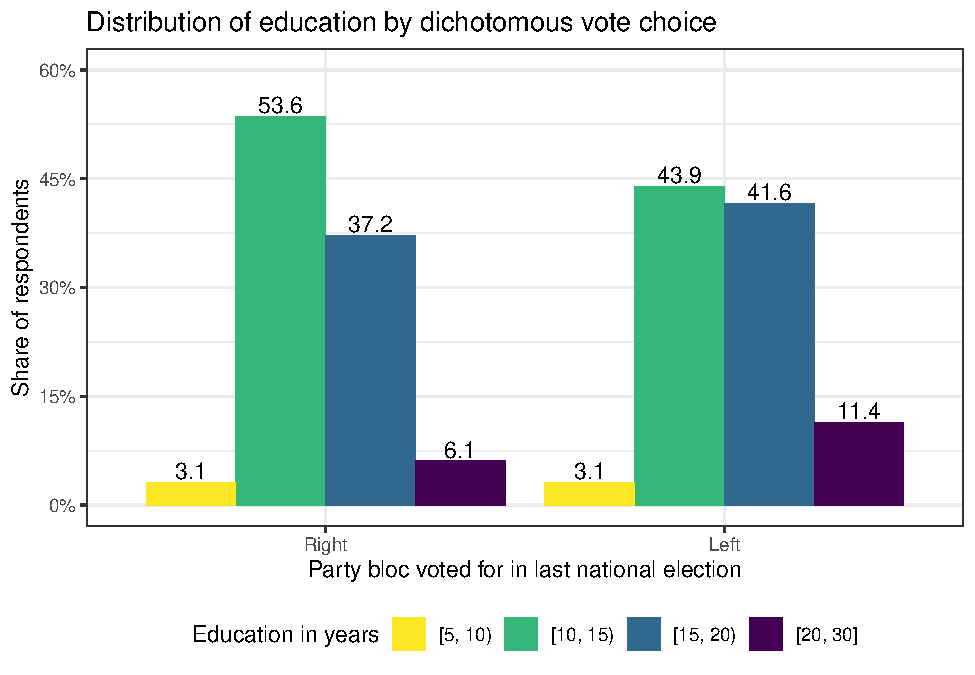
\includegraphics{AVCD-Assignment1-Edenhofer_files/figure-latex/edu-distribution-by-left-right-1} \end{center}

As the graph above shows, the distribution of education varies in two
significant ways between left-bloc voters and right-bloc ones:

\begin{itemize}
\item
  While slightly more than half of all right-bloc voters have between 10
  and 15 years of education, this is only the case for 44\% of left-bloc
  voters.
\item
  The proportion of voters with 20 to 30 years of education is almost
  twice as high among left-bloc voters, compared to their right-bloc
  counterparts.
\end{itemize}

\textcolor{brown}{(b) Estimate the relationship between voting left and years of education. (Hint: use the dummy variable `a-la-Piketty) (c) Make sure to write down your estimation equation formally, and to comment the coefficients (d) Why have you chosen this model? How is it different from an OLS model?}

To estimate the relationship between voting for the left bloc and years
of education, I run a logit model, regressing the dichotomous,
Piketty-esque voting variable on \texttt{eduyrs}. I run a logit model,
as opposed to an OLS one, because the dependent variable is binary.

By way of justification, let us start with the observation that binary
depedent variables imply: \(Y \sim Binom(p).\) We also need to link the
parameter, \(p\), to covariates. One idea would be to express \(p\) as a
linear combination of covariates, \(p = x\beta + \epsilon\), where, in
the general case, \(p\) is n-by-1, \(x\) is n-by-p, \(\beta\) is p-by-1
and \(\epsilon\) is n-by-1. The problem is that this linear probability
model fails the range-matching test: \(p\) is not bounded between zero
and one.

To ensure that for any real-valued set of covariates, \(p\) is bounded
between zero and one, we use the odds, the probability of an event
occurring divided by the probability that it does not occur,
\(\frac{p}{(1-p)}\). The odds can take on any non-negative real number.
As \(p\) increases, the odds increase too. To make sure that the odds
are, indeed, non-negative for any covariate value, we write:
\(\frac{p}{1-p} = exp(\alpha + \beta X)\).

This link of the model parameter, \(p\), to covariates satisfies our
range matching criterion since the exponential function returns positive
real numbers for any real-valued input. Solving this expression for
\(p\) yields:
\(p = \frac{exp(\alpha + \beta X)}{1 + exp(\alpha + \beta X)}\). This
specification is, however, non-linear in the parameters. To linearise,
we use the log - we take the log of the odds (hence, logit),
\(log(\frac{p}{1-p}) = \alpha + \beta X\). This is a linear model, not
of \(E(Y|X)\) (the regression), but of the log of the odds. Thus, logit
models are members of the family of generalised linear
models\footnote{Hence also the \texttt{glm()} command in R.}, where a
non-linear, invertible function, such as \(log(\cdot)\), of the model
parameter(s) is expressed as a linear function of the covariates
(\protect\hyperlink{ref-gailmard_statistical_2014}{Gailmard 2014}).

With these methodological preliminaries in place, we can write our
estimating equation as follows:

\[
log(\frac{VoteLeft_{i}}{1-VoteLeft_{i}}) = \alpha + \beta YearsEducation_{i} + \epsilon_{i} 
\] Here, \(\epsilon\) denotes the error term, while \(\alpha\) captures
the log odds of voting for the left bloc when an individual has zero
years of education. The coefficient of interest is \(\beta\), the
marginal effect of education on the log odds of voting left: the
increase in the log odds of voting left for an additional year of
completed education.

Since we know that the log odds increase if and only if the probability
of voting left increases, we can infer from the sign of \(\hat{\beta}\)
whether or not an additional year of education increases that
probability. We cannot, however, use the coefficient to directly infer
the size of the effect.\footnote{Using
  \(p = \frac{exp(\alpha + \beta X)}{1 + exp(\alpha + \beta X)}\) and
  applying the quotient as well as chain rules of differentiation, it is
  straightforward to see that the marginal effect of education on the
  probability, rather than the log odds, is:
  \(\frac{\partial p}{\partial YearsEducation} = \beta*\frac{exp(\alpha + \beta YearsEducation)}{(1+exp(\alpha + \beta YearsEducation))^2}\).}
To that end, we use predicted probabilities.

In R, we use the \texttt{glm()} function, with the \texttt{family}
argument set to \texttt{binomial}, to estimate the above equation. I
represent the results both via a conventional regression table and a
plot of predicted probabilities obtained via the \texttt{ggpredict()}
function.

\begin{Shaded}
\begin{Highlighting}[]
\CommentTok{\# estimate logit}
\NormalTok{bi\_logit }\OtherTok{\textless{}{-}} \FunctionTok{glm}\NormalTok{(piketty\_dv }\SpecialCharTok{\textasciitilde{}}\NormalTok{ eduyrs, }
                \AttributeTok{family =} \FunctionTok{binomial}\NormalTok{(}\AttributeTok{link =} \StringTok{"logit"}\NormalTok{),}
                \AttributeTok{data =}\NormalTok{ ah21\_mod)}
\CommentTok{\# regression table}
\FunctionTok{modelsummary}\NormalTok{(bi\_logit,}
             \AttributeTok{estimate =} \StringTok{"\{estimate\}\{stars\}"}\NormalTok{, }
             \AttributeTok{coef\_map =} \FunctionTok{c}\NormalTok{(}\StringTok{"eduyrs"} \OtherTok{=} \StringTok{"Years of education"}\NormalTok{),}
             \AttributeTok{output =} \StringTok{"kableExtra"}\NormalTok{,}
             \AttributeTok{title =} \StringTok{"Bivariate logit model"}\NormalTok{) }\SpecialCharTok{\%\textgreater{}\%}
  \FunctionTok{kable\_styling}\NormalTok{(}\AttributeTok{latex\_options =} \StringTok{"hold\_position"}\NormalTok{)}
\end{Highlighting}
\end{Shaded}

\begin{table}[!h]

\caption{\label{tab:bi-logit-table}Bivariate logit model}
\centering
\begin{tabular}[t]{lc}
\toprule
  & (1)\\
\midrule
Years of education & \num{0.082}***\\
 & (\num{0.017})\\
\midrule
Num.Obs. & \num{1324}\\
AIC & \num{1810.5}\\
BIC & \num{1820.8}\\
Log.Lik. & \num{-903.225}\\
F & \num{23.496}\\
RMSE & \num{0.49}\\
\bottomrule
\end{tabular}
\end{table}

Table 3 shows that an additional year of education is
associated\footnote{I wish to stress that this coefficient is unlikely
  to capture the causal effect of education on vote voice, given that we
  do not even control for observed confounders.} with a
significant\footnote{The three stars indicate statistical significance
  at the 1\% level, as explained
  \href{https://vincentarelbundock.github.io/modelsummary/articles/modelsummary.html}{here}.}
increase in the probability of voting for the left bloc. This conclusion
is reinforced by the plot of predicted probabilities below.

\begin{Shaded}
\begin{Highlighting}[]
\CommentTok{\# plot }
\FunctionTok{plot}\NormalTok{(}\FunctionTok{ggpredict}\NormalTok{(bi\_logit, }\AttributeTok{terms=}\StringTok{"eduyrs"}\NormalTok{)) }\SpecialCharTok{+}
  \FunctionTok{labs}\NormalTok{(}\AttributeTok{title =} \StringTok{"Predicted probabilities of voting for left bloc by education (bivariate)"}\NormalTok{, }
       \AttributeTok{y =} \StringTok{"Predicted probability"}\NormalTok{)}
\end{Highlighting}
\end{Shaded}

\begin{center}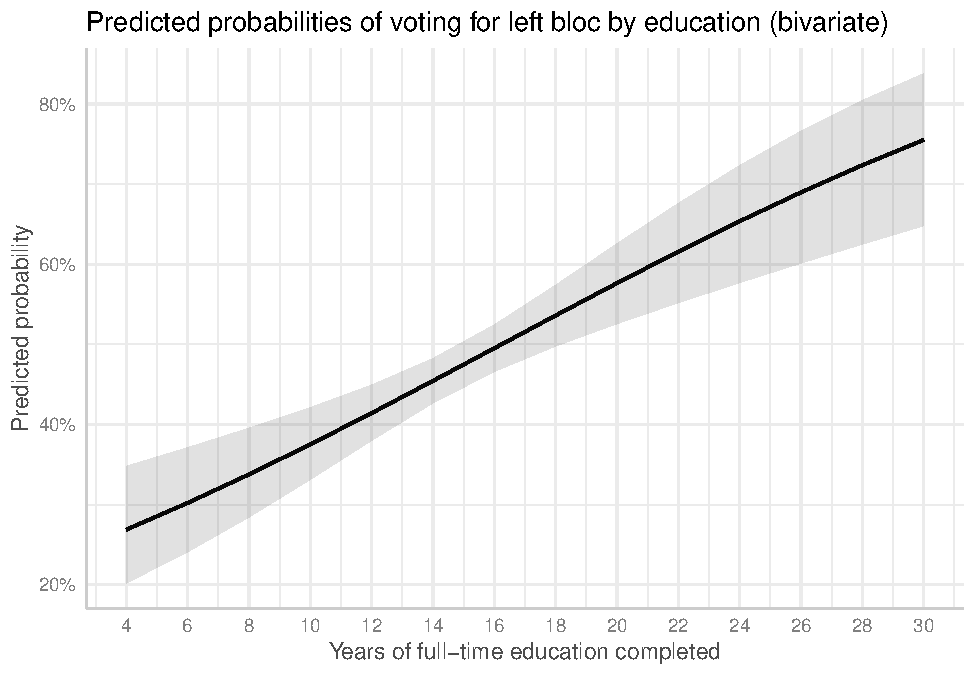
\includegraphics{AVCD-Assignment1-Edenhofer_files/figure-latex/bi-logit-plot-1} \end{center}

\textcolor{brown}{(e) Run the same model again, but adding the socio-economic covariates and controlling for individuals’ level of social capital. Once again, write down the estimation equation formally and do not forget to comment your results after reporting them in a single, tidy table.}

In this model, I will add dummies for gender (\texttt{gendr1}) and
ethnic minority status (\texttt{blgetmg1}). In addition, trust towards
others (\texttt{ppltrst}) will serve as my proxy for social capital, in
line with the arguments developed by Putnam
(\protect\hyperlink{ref-putnam2000bowling}{2000}). My estimating
equation is thus:

\[
log(\frac{VoteLeft_{i}}{1-VoteLeft_{i}}) = \alpha + \beta_{1} YearsEducation_{i} + \beta_{2} Gender_{i} + \beta_{3} EthnicMinority_{i} + \beta_{4} Trust_{i} + \epsilon_{i} 
\]

The estimation of this equation is implemented in R via the following
code, which summarises the results in the form of a regression table.

\begin{Shaded}
\begin{Highlighting}[]
\CommentTok{\# model}
\NormalTok{multi\_logit }\OtherTok{\textless{}{-}} \FunctionTok{glm}\NormalTok{(piketty\_dv }\SpecialCharTok{\textasciitilde{}}\NormalTok{ eduyrs }\SpecialCharTok{+}\NormalTok{ gndr1 }\SpecialCharTok{+}\NormalTok{ blgetmg1 }\SpecialCharTok{+}\NormalTok{ ppltrst, }
                   \AttributeTok{family =} \FunctionTok{binomial}\NormalTok{(}\AttributeTok{link =} \StringTok{"logit"}\NormalTok{),}
                   \AttributeTok{data =}\NormalTok{ ah21\_mod)}

\CommentTok{\# regression table including both models}
\FunctionTok{modelsummary}\NormalTok{(}\FunctionTok{list}\NormalTok{(bi\_logit, multi\_logit),}
             \AttributeTok{estimate =} \StringTok{"\{estimate\}\{stars\}"}\NormalTok{, }
             \AttributeTok{coef\_map =} \FunctionTok{c}\NormalTok{(}\StringTok{"eduyrs"} \OtherTok{=} \StringTok{"Years of education"}\NormalTok{,}
                         \StringTok{"gndr1"} \OtherTok{=} \StringTok{"Gender dummy"}\NormalTok{,}
                         \StringTok{"blgetmg1"} \OtherTok{=} \StringTok{"Ethnic minority dummy"}\NormalTok{,}
                         \StringTok{"ppltrst"} \OtherTok{=} \StringTok{"Trust towards others"}\NormalTok{),}
             \AttributeTok{output =} \StringTok{"kableExtra"}\NormalTok{, }
             \AttributeTok{title =} \StringTok{"Multivariate logit model of voting for the left bloc"}\NormalTok{) }\SpecialCharTok{\%\textgreater{}\%}
  \FunctionTok{kable\_styling}\NormalTok{(}\AttributeTok{latex\_options =} \StringTok{"hold\_position"}\NormalTok{, }\AttributeTok{full\_width =}\NormalTok{ T) }
\end{Highlighting}
\end{Shaded}

\begin{table}[!h]

\caption{\label{tab:multi-logit-table}Multivariate logit model of voting for the left bloc}
\centering
\begin{tabu} to \linewidth {>{\raggedright}X>{\centering}X>{\centering}X}
\toprule
  & (1) & (2)\\
\midrule
Years of education & \num{0.082}*** & \num{0.074}***\\
 & (\num{0.017}) & (\num{0.017})\\
Gender dummy &  & \num{0.047}\\
 &  & (\num{0.113})\\
Ethnic minority dummy &  & \num{0.500}\\
 &  & (\num{0.314})\\
Trust towards others &  & \num{0.071}**\\
 &  & (\num{0.027})\\
\midrule
Num.Obs. & \num{1324} & \num{1321}\\
AIC & \num{1810.5} & \num{1802.8}\\
BIC & \num{1820.8} & \num{1828.7}\\
Log.Lik. & \num{-903.225} & \num{-896.382}\\
F & \num{23.496} & \num{8.122}\\
RMSE & \num{0.49} & \num{0.49}\\
\bottomrule
\end{tabu}
\end{table}

Table 4 demonstrates\footnote{Furthermore, the coefficient for the
  `Gender dummy' captures the difference in voting for the left between
  men and women, which is not statistically significant. Similarly, the
  coefficient for the `Ethnic minority dummy' captures the difference in
  voting for the left between those belonging to a minority, compared to
  those who do not. The difference is not statistically significant.
  `Trust towards others' is a proxy for social capital; those who are
  more trusting are, ceteris paribus, also significantly more likely to
  vote for the left bloc.} that education remains a statistically
significant\footnote{Significant at the 1\% level.} predictor of voting
for the left bloc, even after we control for gender, ethnic minority
status and social capital. In substantive terms, the coefficient
estimate implies that an additional year of education is, ceteris
paribus, associated with an increase in the odds\footnote{This is
  obtained by computing \texttt{100*(exp(0.074)-1)}.} of voting for the
left bloc by 7.7\%. This conclusion is, as above, reinforced by the plot
of predicted probabilities below.\footnote{As noted above, the marginal
  effects and, thus, also the predicted probabilities depend on the
  values of the other covariates. The \texttt{ggpredict()} function sets
  the values of all non-education covariates equal to their mean value.}

\begin{Shaded}
\begin{Highlighting}[]
\CommentTok{\# predicted probability }
\FunctionTok{plot}\NormalTok{(}\FunctionTok{ggpredict}\NormalTok{(multi\_logit, }\AttributeTok{terms =} \StringTok{"eduyrs"}\NormalTok{)) }\SpecialCharTok{+}
  \FunctionTok{labs}\NormalTok{(}\AttributeTok{title =} \StringTok{"Predicted probabilities of voting}\SpecialCharTok{\textbackslash{}n}\StringTok{for left bloc by education (multivariate model)"}\NormalTok{, }
       \AttributeTok{y =} \StringTok{"Predicted probability"}\NormalTok{)}
\end{Highlighting}
\end{Shaded}

\begin{center}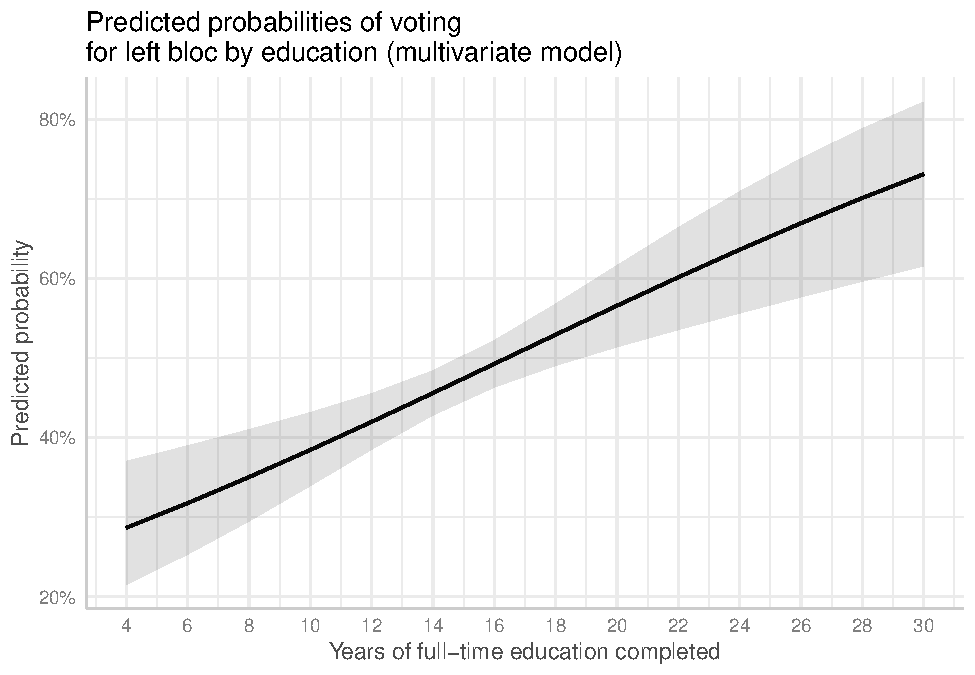
\includegraphics{AVCD-Assignment1-Edenhofer_files/figure-latex/multi-logit-plot-1} \end{center}

\hypertarget{section-2}{%
\subsection{1.3}\label{section-2}}

\textcolor{brown}{(a) Look back at your results in Exercise 1.2, comment them, and explain how they relate to Abou-Chadi and Hix (2021).}

By way of recap, the two key results of the preceding section are:

\begin{itemize}
\item
  The share of those with 20 to 30 years of education among left-bloc
  voters is almost twice as high as the share among right-bloc voters.
\item
  There is a positive association between years of education and the
  probability of voting for the left bloc, which is robust to the
  inclusion of the socio-demographic covariates contained in the
  dataset.
\end{itemize}

Broadly speaking, these results are consistent with figure 1 in
Abou-Chadi and Hix
(\protect\hyperlink{ref-abou-chadi_brahmin_2021}{2021}), though there is
an important difference. Using a categorical measure of education, the
authors find a non-linear effect of education on left-right vote choice.
In our case, the coefficient estimate on the square of years of
education is insignificant (see table 11 in the appendix), implying that
the effect is positive and linear.

Conceptually, our results are based on what Abou-Chadi and Hix
(\protect\hyperlink{ref-abou-chadi_brahmin_2021}{2021}) argue is the
``wrong'' kind of dependent variable, namely a dichotomous measure of
vote choice. Such measures, the authors submit, fail to account for the
growing fragmentation of party systems in Western European countries
over the last three decades (e.g.
\protect\hyperlink{ref-chiaramonte2019towards}{Chiaramonte and Emanuele
2019}). As a result, analyses resting on binary dependent variables of
vote choice do not allow us to say anything about the ``mechanisms'' of
this association. Using a more fine-grained dependent variable,
Abou-Chadi and Hix
(\protect\hyperlink{ref-abou-chadi_brahmin_2021}{2021}) conclude that
the positive association between education and left-wing support is
driven by more educated individuals being more likely to vote for
left-libertarian, as opposed to mainstream left, parties.

\textcolor{brown}{(b) Does education matter? Why? Take into consideration one possible channel through which education affects voting behaviour. Make sure to discuss whether it is a compositional or a contextual effect, that is, whether individuals with certain political attitudes and preferences self-select into/out of education, or whether education shapes and changes political attitudes and preferences.}

In (most) advanced industrial democracies, education matters greatly for
explaining vote choice in at least two ways. First, as Abou-Chadi and
Hix (\protect\hyperlink{ref-abou-chadi_brahmin_2021}{2021}) show, more
educated individuals are more likely to support left-libertarian
parties, particularly green ones. Secondly, the authors show that
``higher educated voters who are in favor of redistribution are more
than 30\% more likely to support a party of the left than a party of the
right. {[}\ldots{]} for those ``Brahmin'' who decide to vote for the
left, a key reason for doing so is that they support economic
redistribution.''
(\protect\hyperlink{ref-abou-chadi_brahmin_2021}{Abou-Chadi and Hix
2021, 88}) That is, when educated individuals hold pro-redistribution
preferences, these are a strong motivation for supporting left parties.

Delving deeper into the mechanisms underlying the positive relationship
between education and left-wing voting suggests two types of mechanisms
are at work. First, education can causally change individuals'
preferences and beliefs. Given that people strategically choose how much
education to obtain (self-selection), this mechanism is hard, albeit not
impossible, to evaluate empirically. Indeed, several studies exploit
compulsory schooling reforms to tease out the causal effect of education
on social attitudes and political preferences. Employing such an
empirical strategy, Cavaille and Marshall
(\protect\hyperlink{ref-cavaille2019education}{2019}), for instance,
find that higher education reduces anti-immigrant sentiment, while Yang
(\protect\hyperlink{ref-yang2022more}{2022}) finds that more schooling
reduces prejudices against sexual minorities. These studies therefore
suggest that education affects individuals' values, beliefs and
preferences in ways that make them more likely to support left-wing,
especially left-libertarian, parties.

A second mechanism, however, is at work, namely self-selection into and
out of education. That is, we would expect individuals who are ex ante
more likely to gain from higher education to strategically choose to
obtain more of it, whereas those who are less likely to gain by virtue
of, for example, lower motivation, will obtain less education.
Self-selection matters for vote choice since (some of) the factors that
lead individuals to obtain more/less education are likely correlated
with determinants of vote choice, thus confounding the relationship
between education and the latter. Individuals who are more willing to
expose themselves to new influences may, for instance, be more likely to
attend university, but also view immigration more favourably and, as a
result, vote for left-libertarian parties. In that case, it is not
education that causes individuals to vote for these parties, but their
pre-existing attitudes that explain both university attendance and vote
choice.

While I believe there is solid evidence for the causal effect of
education on political preferences and behaviour, the effect sizes are
small. Moreover, in no Western European country does university
attendance significantly exceed 50\%, suggesting substantial room for
self-selection into and out of education, as, indeed, theories of human
capital accumulation would lead us to predict
(\protect\hyperlink{ref-becker2009human}{Becker 2009}). Hence, I think
that a substantial portion, if not most of it, of the association
between education and vote choice is non-causal, i.e.~driven by
self-selection.

\hypertarget{exercise-2}{%
\section{Exercise 2}\label{exercise-2}}

\hypertarget{section-3}{%
\subsection{2.1-2.2}\label{section-3}}

\textcolor{brown}{You shall keep using the same dataset from the previous exercise. Test whether there is a positive relationship between voting the Libertarian Left and years of education. Is the aforementioned relationship stronger than that between education and voting for the Mainstream Left? Compare the two specifications in the same tidy table, and explain which criteria you have used in your assessment.}

As in exercise 1, I use a logit model to estimate the relationship
between the \texttt{lib\_left\_dummy} and \texttt{eduyrs}, with the
dependent variable being unity when an individual voted for the Greens
in the last election and zero otherwise. The result is reported in table
5, along with the results obtained above for the Piketty-like dependent
variable.

\begin{Shaded}
\begin{Highlighting}[]
\CommentTok{\# libertarian left dummy }
\NormalTok{ah21\_mod }\OtherTok{\textless{}{-}}\NormalTok{ ah21\_mod }\SpecialCharTok{\%\textgreater{}\%}
  \FunctionTok{mutate}\NormalTok{(}\AttributeTok{lib\_left\_dummy =} \FunctionTok{ifelse}\NormalTok{(prtvede1 }\SpecialCharTok{==} \DecValTok{4}\NormalTok{, }\DecValTok{1}\NormalTok{, }\DecValTok{0}\NormalTok{)) }\CommentTok{\# 1 for Greens, 0 otherwise}

\CommentTok{\# logit model }
\NormalTok{bi\_logit\_lib\_left }\OtherTok{\textless{}{-}} \FunctionTok{glm}\NormalTok{(lib\_left\_dummy }\SpecialCharTok{\textasciitilde{}}\NormalTok{ eduyrs, }
                         \AttributeTok{family =} \FunctionTok{binomial}\NormalTok{(}\AttributeTok{link =} \StringTok{"logit"}\NormalTok{), }
                         \AttributeTok{data =}\NormalTok{ ah21\_mod)}

\CommentTok{\# regression table }
\NormalTok{models1 }\OtherTok{\textless{}{-}} \FunctionTok{list}\NormalTok{(}\StringTok{"Right vs. left bloc"} \OtherTok{=}\NormalTok{ bi\_logit, }
                \StringTok{"Left libertarian vs. rest"} \OtherTok{=}\NormalTok{ bi\_logit\_lib\_left)}
\FunctionTok{modelsummary}\NormalTok{(models1, }
             \AttributeTok{estimate =} \StringTok{"\{estimate\}\{stars\}"}\NormalTok{, }
             \AttributeTok{coef\_map =} \FunctionTok{c}\NormalTok{(}\StringTok{"eduyrs"} \OtherTok{=} \StringTok{"Years of education"}\NormalTok{), }
             \AttributeTok{output =} \StringTok{"kableExtra"}\NormalTok{, }
             \AttributeTok{title =} \StringTok{"Comparing the effect of education (bivariate case)"}\NormalTok{) }\SpecialCharTok{\%\textgreater{}\%}
  \FunctionTok{kable\_styling}\NormalTok{(}\AttributeTok{latex\_options =} \StringTok{"hold\_position"}\NormalTok{, }\AttributeTok{full\_width =}\NormalTok{ T)}
\end{Highlighting}
\end{Shaded}

\begin{table}[!h]

\caption{\label{tab:lib-left-logit-comp}Comparing the effect of education (bivariate case)}
\centering
\begin{tabu} to \linewidth {>{\raggedright}X>{\centering}X>{\centering}X}
\toprule
  & Right vs. left bloc & Left libertarian vs. rest\\
\midrule
Years of education & \num{0.082}*** & \num{0.130}***\\
 & (\num{0.017}) & (\num{0.021})\\
\midrule
Num.Obs. & \num{1324} & \num{1324}\\
AIC & \num{1810.5} & \num{1167.5}\\
BIC & \num{1820.8} & \num{1177.9}\\
Log.Lik. & \num{-903.225} & \num{-581.760}\\
F & \num{23.496} & \num{36.847}\\
RMSE & \num{0.49} & \num{0.37}\\
\bottomrule
\end{tabu}
\end{table}

Education, as table 5 bears out, is significantly\footnote{Significant
  at the 1\% level} associated with both voting for the left bloc and
for the Greens, the left-libertarian party, though the association is
stronger for the latter than for the former. Substantively, an
additional year of education is associated with an increase\footnote{As
  explained above, these values are obtained by computing
  \texttt{100*(exp(0.082)-1)} and \texttt{100*(exp(0.13)-1)}.} in the
odds of voting for the left bloc by approximately 8.5\%, whereas the
increase is 13.9\% for the Greens.

\hypertarget{section-4}{%
\subsection{2.3}\label{section-4}}

\textcolor{brown}{Restrict the dataset to left-wing voters. Are preferences for income redistribution a good predictor of voting for both the Mainstream Left and the Libertarian Left? Compare your results (again, in the same table, if possible), and discuss them.}

To restrict the dataset to left-wing voters, I consider only voters who
voted for the SPD (\texttt{prtvede1\ ==\ 2}) or the Greens
(\texttt{prtvede1\ ==\ 4}) since these are the only left-wing parties
listed in table 1 of the online appendix
(\protect\hyperlink{ref-abou-chadi_brahmin_2021}{Abou-Chadi and Hix
2021}). Then, I regress \texttt{m\_left\_dummy} and
\texttt{left\_lib\_dummy} respectively on \texttt{gincdif}, and estimate
these specifications via a logit model. In these two models,
respondents' (dis)agreement with the statement that `government should
reduce income differences' serves as our proxy for attitudes towards
redistribution (\texttt{gincdif}).

\begin{Shaded}
\begin{Highlighting}[]
\CommentTok{\# prune data to left{-}wing voters only}
\NormalTok{ah21\_mod\_left }\OtherTok{\textless{}{-}}\NormalTok{ ah21\_mod }\SpecialCharTok{\%\textgreater{}\%}
  \FunctionTok{filter}\NormalTok{(prtvede1 }\SpecialCharTok{\%in\%} \FunctionTok{c}\NormalTok{(}\DecValTok{2}\NormalTok{, }\DecValTok{4}\NormalTok{)) }\SpecialCharTok{\%\textgreater{}\%} \CommentTok{\# Greens and SPD }
  \FunctionTok{mutate}\NormalTok{(}\AttributeTok{left\_lib\_dummy =} \FunctionTok{ifelse}\NormalTok{(prtvede1 }\SpecialCharTok{==} \DecValTok{4}\NormalTok{, }\DecValTok{1}\NormalTok{, }\DecValTok{0}\NormalTok{), }\CommentTok{\# Greens}
         \AttributeTok{m\_left\_dummy =} \FunctionTok{ifelse}\NormalTok{(prtvede1 }\SpecialCharTok{==} \DecValTok{2}\NormalTok{, }\DecValTok{1}\NormalTok{, }\DecValTok{0}\NormalTok{)) }\CommentTok{\# SPD}

\CommentTok{\# models }
\NormalTok{bi\_logit\_re\_ml }\OtherTok{\textless{}{-}} \FunctionTok{glm}\NormalTok{(m\_left\_dummy }\SpecialCharTok{\textasciitilde{}}\NormalTok{ gincdif, }
                      \AttributeTok{family =} \FunctionTok{binomial}\NormalTok{(}\AttributeTok{link =} \StringTok{"logit"}\NormalTok{), }
                      \AttributeTok{data =}\NormalTok{ ah21\_mod\_left)}
\NormalTok{bi\_logit\_re\_ll }\OtherTok{\textless{}{-}} \FunctionTok{glm}\NormalTok{(left\_lib\_dummy }\SpecialCharTok{\textasciitilde{}}\NormalTok{ gincdif, }
                      \AttributeTok{family =} \FunctionTok{binomial}\NormalTok{(}\AttributeTok{link =} \StringTok{"logit"}\NormalTok{), }
                      \AttributeTok{data =}\NormalTok{ ah21\_mod\_left)}

\CommentTok{\# modelsummary}
\NormalTok{models2 }\OtherTok{\textless{}{-}} \FunctionTok{list}\NormalTok{(}\StringTok{"Mainstream left (SPD)"} \OtherTok{=}\NormalTok{ bi\_logit\_re\_ml, }
                \StringTok{"Left libertarian (Greens)"} \OtherTok{=}\NormalTok{ bi\_logit\_re\_ll)}
\CommentTok{\# table }
\FunctionTok{modelsummary}\NormalTok{(models2, }
             \AttributeTok{estimate =} \StringTok{"\{estimate\}\{stars\}"}\NormalTok{,}
             \AttributeTok{coef\_map =} \FunctionTok{c}\NormalTok{(}\StringTok{"gincdif"} \OtherTok{=} \StringTok{"Gov\textquotesingle{}t should reduce income differences"}\NormalTok{), }
             \AttributeTok{title =} \StringTok{"Attitudes towards redistribution as predictor of vote choice among left{-}wing voters (bivariate)"}\NormalTok{, }
             \AttributeTok{output =} \StringTok{"kableExtra"}\NormalTok{) }\SpecialCharTok{\%\textgreater{}\%}
  \FunctionTok{kable\_styling}\NormalTok{(}\AttributeTok{latex\_options =} \StringTok{"hold\_position"}\NormalTok{, }\AttributeTok{full\_width =}\NormalTok{ T) }\SpecialCharTok{\%\textgreater{}\%}
  \FunctionTok{add\_footnote}\NormalTok{(}\AttributeTok{label =} \StringTok{"See footnote 3 for interpreting the explanatory variable."}\NormalTok{, }
               \AttributeTok{notation =} \StringTok{"none"}\NormalTok{)}
\end{Highlighting}
\end{Shaded}

\begin{table}[!h]

\caption{\label{tab:left-wing-vot-comp}Attitudes towards redistribution as predictor of vote choice among left-wing voters (bivariate)}
\centering
\begin{tabu} to \linewidth {>{\raggedright}X>{\centering}X>{\centering}X}
\toprule
  & Mainstream left (SPD) & Left libertarian (Greens)\\
\midrule
Gov't should reduce income differences & \num{-0.022} & \num{0.022}\\
 & (\num{0.094}) & (\num{0.094})\\
\midrule
Num.Obs. & \num{623} & \num{623}\\
AIC & \num{816.6} & \num{816.6}\\
BIC & \num{825.5} & \num{825.5}\\
Log.Lik. & \num{-406.311} & \num{-406.311}\\
F & \num{0.053} & \num{0.053}\\
RMSE & \num{0.48} & \num{0.48}\\
\bottomrule
\multicolumn{3}{l}{\textsuperscript{} See footnote 3 for interpreting the explanatory variable.}\\
\end{tabu}
\end{table}

Table 6 shows that - when restricting the data only two left-wing voters
- attitudes towards redistribution are not a statistically significant
predictor of vote choice. This does not imply, it is worth noting, that
redistributive preferences do not affect the probability of supporting
left-wing parties in general (i.e.~among all voters).\footnote{Table 12
  in the appendix demonstrates this point explicitly. In models (2) and
  (3), redistributive attitudes are strongly predictive of voting for
  the left bloc.} Instead, this result is best interpreted as showing
that those with relatively strong preferences for redistribution
`select' into the left electorate. As a result, redistributive
preferences do not vary all that much among left-wing voters, explaining
our `null' finding.

\hypertarget{section-5}{%
\subsection{2.4}\label{section-5}}

\textcolor{brown}{What happens when you add attitudes towards immigrants and sexual minorities as covariates? (a) Report the estimation equation formally, (b) Comment the coefficients, reporting the two model specifications in the same, tidy table, (c) What do you learn from this? Are preferences for redistribution always a good predictor of left voting?}

I will run two logit models - one with \texttt{m\_left\_dummy} as the
dependent variable, and the other with \texttt{left\_lib\_dummy}.
Letting \(p\) denote the respective probabilities, we can write the
estimating equation as follows:

\[
log(\frac{p_{i}}{1-p_{i}}) = \alpha + \beta_{1} YearsEducation_{i} + \beta_{2} Gender_{i} + \beta_{3} ImmigrantSentiment_{i} + \beta_{4} LGBT_{i} + \epsilon_{i}
\]

As above, our main coefficient of interest is \(\beta_{1}\), which
represents the marginal effect of an additional year on education on the
log odds of voting for the mainstream left or left-libertarian parties,
holding all other variables constant. Formally, we can write this as:

\[
\frac{\partial log(\frac{p_{i}}{1-p_{i}})}{\partial YearsEducation} = \beta_{1}
\]

More intuitively, we can interpret \(100*(exp(\beta_{1})-1)\) as the
percent change in the odds for an additional year of education. The
interpretation of all other coefficients is analogous. They all
represent partial derivatives.

In R, I estimate this equation by running:

\begin{Shaded}
\begin{Highlighting}[]
\CommentTok{\# models }
\NormalTok{bi\_logit\_re\_ml\_m }\OtherTok{\textless{}{-}} \FunctionTok{glm}\NormalTok{(m\_left\_dummy }\SpecialCharTok{\textasciitilde{}}\NormalTok{ gincdif }\SpecialCharTok{+}\NormalTok{ imwbcnt }\SpecialCharTok{+}\NormalTok{ freehms, }
                      \AttributeTok{family =} \FunctionTok{binomial}\NormalTok{(}\AttributeTok{link =} \StringTok{"logit"}\NormalTok{), }
                      \AttributeTok{data =}\NormalTok{ ah21\_mod\_left)}
\NormalTok{bi\_logit\_re\_ll\_m }\OtherTok{\textless{}{-}} \FunctionTok{glm}\NormalTok{(left\_lib\_dummy }\SpecialCharTok{\textasciitilde{}}\NormalTok{ gincdif }\SpecialCharTok{+}\NormalTok{ gincdif }\SpecialCharTok{+}\NormalTok{ imwbcnt }\SpecialCharTok{+}\NormalTok{ freehms, }
                      \AttributeTok{family =} \FunctionTok{binomial}\NormalTok{(}\AttributeTok{link =} \StringTok{"logit"}\NormalTok{), }
                      \AttributeTok{data =}\NormalTok{ ah21\_mod\_left)}

\CommentTok{\# modelsummary}
\NormalTok{models3 }\OtherTok{\textless{}{-}} \FunctionTok{list}\NormalTok{(}\StringTok{"Mainstream left (SPD)"} \OtherTok{=}\NormalTok{ bi\_logit\_re\_ml\_m, }
                \StringTok{"Left libertarian (Greens)"} \OtherTok{=}\NormalTok{ bi\_logit\_re\_ll\_m)}
\CommentTok{\# table }
\FunctionTok{modelsummary}\NormalTok{(models3, }
             \AttributeTok{estimate =} \StringTok{"\{estimate\}\{stars\}"}\NormalTok{,}
             \AttributeTok{coef\_map =} \FunctionTok{c}\NormalTok{(}\StringTok{"gincdif"} \OtherTok{=} \StringTok{"Gov\textquotesingle{}t should reduce income differences"}\NormalTok{,}
                          \StringTok{"imwbcnt"} \OtherTok{=} \StringTok{"Immigrants make country worse/better place to live"}\NormalTok{, }
                          \StringTok{"freehms"} \OtherTok{=} \StringTok{"LBGT+ people should be free to live as they wish"}\NormalTok{), }
             \AttributeTok{title =} \StringTok{"Attitudes towards redistribution as predictor of vote choice among left{-}wing voters (multivariate)"}\NormalTok{, }
             \AttributeTok{output =} \StringTok{"kableExtra"}\NormalTok{) }\SpecialCharTok{\%\textgreater{}\%}
  \FunctionTok{kable\_styling}\NormalTok{(}\AttributeTok{latex\_options =} \StringTok{"hold\_position"}\NormalTok{, }\AttributeTok{full\_width =}\NormalTok{ T) }
\end{Highlighting}
\end{Shaded}

\begin{table}[!h]

\caption{\label{tab:left-wing-vot-comp-multi}Attitudes towards redistribution as predictor of vote choice among left-wing voters (multivariate)}
\centering
\begin{tabu} to \linewidth {>{\raggedright}X>{\centering}X>{\centering}X}
\toprule
  & Mainstream left (SPD) & Left libertarian (Greens)\\
\midrule
Gov't should reduce income differences & \num{-0.145} & \num{0.145}\\
 & (\num{0.101}) & (\num{0.101})\\
Immigrants make country worse/better place to live & \num{-0.219}*** & \num{0.219}***\\
 & (\num{0.047}) & (\num{0.047})\\
LBGT+ people should be free to live as they wish & \num{0.650}*** & \num{-0.650}***\\
 & (\num{0.155}) & (\num{0.155})\\
\midrule
Num.Obs. & \num{622} & \num{622}\\
AIC & \num{762.9} & \num{762.9}\\
BIC & \num{780.6} & \num{780.6}\\
Log.Lik. & \num{-377.439} & \num{-377.439}\\
F & \num{15.213} & \num{15.213}\\
RMSE & \num{0.46} & \num{0.46}\\
\bottomrule
\end{tabu}
\end{table}

As before, the coefficient estimate on redistributive preferences is not
statistically significant, suggesting that, among left-wing voters,
redistributive preferences are not a strong predictor of which type of
left-wing party they vote for.\footnote{See table 12 in the appendix,
  which shows that, among all voters, redistributive attitudes do
  significantly predict left-bloc vote choice, even after controlling
  for socio-demographic and attitudinal variables.} This suggests that
individuals with strong redistributive preferences select into the left
party bloc, but other variables then determine which left party they
vote for.

\hypertarget{section-6}{%
\subsection{2.5}\label{section-6}}

\textcolor{brown}{(a) Go back to the main dataset: you want to explore the relationship between preferences for redistribution and voting behavior in general: (a) What model would you want to run? And why? (b) Run the appropriate model (with and without the aforementioned attitudinal covariates) and report your baseline category of choice. What is the point of having a baseline category? Why do MNL models have it while logit models do not?}

Exploring the relationship between redistributive preferences and voting
behaviour in general is best done by means of a multinomial model, which
accounts for our dependent variable being an unordered categorical
variable consisting of the different parties. Multinomial models
therefore address one shortcoming of logit models. With an unordered
categorical variable (with more than two levels), we can only estimate a
logit model by collapsing this variable. This is potentially problematic
since our reference group (the ``zero'' group) may consist of highly
heterogeneous entities, rendering a substantively meaningful
interpretation difficult, if not impossible.

To see this, suppose we regressed a dummy for SPD voting on
redistributive preferences and found a positive coefficient. The
interpretation would then be that a stronger preference for
redistribution increases the probability of voting for the SPD, relative
to not doing so. But ``not doing so'' includes voting for the CDU/CSU,
FDP, NPD, LINKE or AfD - a highly disparate group of parties.

Hence, I will run two multinomial models without and with attitudinal
covariates, where my reference category is voting for the SPD - the
mainstream left party. Given that multinomial models have multi-valued
categorical variable as their dependent variables, they require a
reference category, unlike logit models, where the reference group is
the ``zero'' group. I choose this reference category because the debate
between Piketty, on the one hand, and Abou-Chadi and Hix, on the other,
mainly concerns the fortunes of this party family.

In R, I estimate the models via the following code. Given the relatively
complex output of the \texttt{multinom()} function, I only represent the
coefficient estimates for \texttt{gincdif}, and do so for each model
separately.\footnote{Unfortunately, I have not been able to suppress the
  messages printed by \texttt{multinom()}.}

\begin{Shaded}
\begin{Highlighting}[]
\CommentTok{\# set SPD reference category }
\NormalTok{ah21}\SpecialCharTok{$}\NormalTok{prtvede11 }\OtherTok{\textless{}{-}} \FunctionTok{relevel}\NormalTok{(}\FunctionTok{factor}\NormalTok{(ah21}\SpecialCharTok{$}\NormalTok{prtvede1), }\AttributeTok{ref =} \StringTok{\textquotesingle{}2\textquotesingle{}}\NormalTok{)}

\CommentTok{\# estimate models }
\NormalTok{multinom1 }\OtherTok{\textless{}{-}} \FunctionTok{multinom}\NormalTok{(prtvede11 }\SpecialCharTok{\textasciitilde{}}\NormalTok{ gincdif, }
                      \AttributeTok{data =}\NormalTok{ ah21)}
\end{Highlighting}
\end{Shaded}

\hypertarget{weights-24-14-variable}{%
\section{weights: 24 (14 variable)}\label{weights-24-14-variable}}

initial value 3177.386676 iter 10 value 2501.351614 iter 20 value
2313.757002 iter 30 value 2311.405825 iter 40 value 2311.127502 iter 50
value 2310.830344 final value 2310.821418 converged

\begin{Shaded}
\begin{Highlighting}[]
\NormalTok{multinom2 }\OtherTok{\textless{}{-}} \FunctionTok{multinom}\NormalTok{(prtvede11 }\SpecialCharTok{\textasciitilde{}}\NormalTok{ gincdif }\SpecialCharTok{+}\NormalTok{ freehms }\SpecialCharTok{+}\NormalTok{ imwbcnt,}
                      \AttributeTok{data =}\NormalTok{ ah21)}
\end{Highlighting}
\end{Shaded}

\hypertarget{weights-40-28-variable}{%
\section{weights: 40 (28 variable)}\label{weights-40-28-variable}}

initial value 3146.195053 iter 10 value 2397.929738 iter 20 value
2193.150798 iter 30 value 2141.544175 iter 40 value 2133.250099 iter 50
value 2132.805092 iter 60 value 2132.691336 iter 70 value 2132.676187
iter 80 value 2132.668315 iter 90 value 2132.665554 iter 100 value
2132.659997 final value 2132.659997 stopped after 100 iterations

\begin{Shaded}
\begin{Highlighting}[]
\NormalTok{models3 }\OtherTok{\textless{}{-}} \FunctionTok{list}\NormalTok{(multinom1, multinom2)}


\CommentTok{\# loop for printing out tables}
\ControlFlowTok{for}\NormalTok{(i }\ControlFlowTok{in} \FunctionTok{c}\NormalTok{(}\DecValTok{1}\SpecialCharTok{:}\DecValTok{2}\NormalTok{))\{}
\NormalTok{  dd }\OtherTok{\textless{}{-}} \FunctionTok{modelsummary}\NormalTok{(models3[[i]],}
             \AttributeTok{estimate =} \StringTok{"\{estimate\}\{stars\}"}\NormalTok{, }
             \AttributeTok{coef\_map =} \FunctionTok{c}\NormalTok{(}\StringTok{"gincdif"} \OtherTok{=} \StringTok{"Attitudes towards redistribution"}\NormalTok{,}
                         \StringTok{"feehms"} \OtherTok{=} \StringTok{"LGBT+ people should be free to live as they wish"}\NormalTok{,}
                         \StringTok{"imwbcnt"} \OtherTok{=} \StringTok{"Immigrants make the country a worse/better place to live"}\NormalTok{),}
             \AttributeTok{output =} \StringTok{"data.frame"}\NormalTok{) }\SpecialCharTok{\%\textgreater{}\%} 
  \FunctionTok{filter}\NormalTok{(}\FunctionTok{grepl}\NormalTok{(}\StringTok{"Attitudes towards redistribution"}\NormalTok{, term), }
         \FunctionTok{grepl}\NormalTok{(}\StringTok{"estimate"}\NormalTok{, statistic)) }
\CommentTok{\# add rownames, derived from ESS codebook (CDU/CSU = 1, LINKE = 3, Greens = 4, FDP = 5, AfD = 6, Pirates = 7, NPD = 8)}
\FunctionTok{rownames}\NormalTok{(dd) }\OtherTok{\textless{}{-}} \FunctionTok{c}\NormalTok{(}\StringTok{"CDU/CSU"}\NormalTok{, }\StringTok{"LINKE"}\NormalTok{, }\StringTok{"Greens"}\NormalTok{, }\StringTok{"FDP"}\NormalTok{, }\StringTok{"AfD"}\NormalTok{, }\StringTok{"Pirates"}\NormalTok{, }\StringTok{"NPD"}\NormalTok{)}
\NormalTok{dd }\OtherTok{\textless{}{-}}\NormalTok{ dd }\SpecialCharTok{\%\textgreater{}\%}
  \FunctionTok{select}\NormalTok{(}\SpecialCharTok{{-}}\DecValTok{1}\NormalTok{) }\SpecialCharTok{\%\textgreater{}\%}
  \FunctionTok{kbl}\NormalTok{(}\AttributeTok{booktabs =}\NormalTok{ T, }
      \AttributeTok{caption =} \FunctionTok{paste0}\NormalTok{(}\StringTok{"Attitudes towards redistribution based on model "}\NormalTok{, i)) }\SpecialCharTok{\%\textgreater{}\%}
  \FunctionTok{kable\_styling}\NormalTok{(}\AttributeTok{full\_width =}\NormalTok{ T)}
\FunctionTok{print}\NormalTok{(dd)}
\NormalTok{\}}
\end{Highlighting}
\end{Shaded}

\begin{table}

\caption{\label{tab:multinomial-model}Attitudes towards redistribution based on model 1}
\centering
\begin{tabu} to \linewidth {>{\raggedright}X>{\raggedright}X>{\raggedright}X>{\raggedright}X}
\toprule
  & term & statistic & (1)\\
\midrule
CDU/CSU & Attitudes towards redistribution & estimate & -0.498***\\
LINKE & Attitudes towards redistribution & estimate & -10.856***\\
Greens & Attitudes towards redistribution & estimate & 0.021\\
FDP & Attitudes towards redistribution & estimate & 0.045\\
AfD & Attitudes towards redistribution & estimate & 0.248*\\
\addlinespace
Pirates & Attitudes towards redistribution & estimate & 0.411***\\
NPD & Attitudes towards redistribution & estimate & 0.533***\\
\bottomrule
\end{tabu}
\end{table}
\begin{table}

\caption{\label{tab:multinomial-model}Attitudes towards redistribution based on model 2}
\centering
\begin{tabu} to \linewidth {>{\raggedright}X>{\raggedright}X>{\raggedright}X>{\raggedright}X}
\toprule
  & term & statistic & (1)\\
\midrule
CDU/CSU & Attitudes towards redistribution & estimate & -0.484**\\
LINKE & Attitudes towards redistribution & estimate & -12.947***\\
Greens & Attitudes towards redistribution & estimate & 0.004\\
FDP & Attitudes towards redistribution & estimate & 0.110\\
AfD & Attitudes towards redistribution & estimate & 0.279*\\
\addlinespace
Pirates & Attitudes towards redistribution & estimate & 0.398***\\
NPD & Attitudes towards redistribution & estimate & 0.551***\\
\bottomrule
\end{tabu}
\end{table}

Finally, let us briefly interpret the coefficient estimates. Since I
have not rescaled the redistributive preference variable an increase in
the latter, recall, amounts to less support for redistribution. So, the
statistically significant coefficient estimates on CDU/CSU and LINKE
mean that, as individuals become less supportive of redistribution, they
are less likely to vote for these two parties, relative to voting for
the SPD. The effect is particularly pronounced for the LINKE, suggesting
that people with moderate redistributive preferences are, ceteris
paribus, much more likely to vote for the SPD than for the LINKE.
Positive coefficient estimates, by contrast, mean that, as individuals
become less supportive of redistribution, they are more likely to vote
for the AfD, the NPD, or the Pirates, relative to voting for the SPD.
When comparing the SPD to the FDP and Greens, there is no significant
effect of redistributive preferences on vote choice.

\hypertarget{appendix}{%
\section{Appendix}\label{appendix}}

\hypertarget{exercise-1-1}{%
\subsection{Exercise 1}\label{exercise-1-1}}

\hypertarget{section-7}{%
\subsubsection{1.1}\label{section-7}}

\begin{Shaded}
\begin{Highlighting}[]
\NormalTok{ah21 }\SpecialCharTok{\%\textgreater{}\%}
  \FunctionTok{select}\NormalTok{(}\SpecialCharTok{{-}}\FunctionTok{c}\NormalTok{(cntry, gndr, gndr1, blgetmg, blgetmg1, prtvede1)) }\SpecialCharTok{\%\textgreater{}\%}
  \FunctionTok{datasummary\_skim}\NormalTok{(}\AttributeTok{output =} \StringTok{"kableExtra"}\NormalTok{, }
                   \AttributeTok{title =} \StringTok{"Summary statistics for ordered categorical variables"}\NormalTok{) }\SpecialCharTok{\%\textgreater{}\%}
  \FunctionTok{kable\_styling}\NormalTok{(}\AttributeTok{latex\_options =} \FunctionTok{c}\NormalTok{(}\StringTok{"scale\_down"}\NormalTok{, }\StringTok{"hold\_position"}\NormalTok{))}
\end{Highlighting}
\end{Shaded}

\begin{table}[!h]

\caption{\label{tab:eda-ah21-histo}Summary statistics for ordered categorical variables}
\centering
\resizebox{\linewidth}{!}{
\begin{tabular}[t]{lrrrrrrr>{}r}
\toprule
  & Unique (\#) & Missing (\%) & Mean & SD & Min & Median & Max &   \\
\midrule
Most people can be trusted or you can't be too careful & 11 & 0 & \num{5.6} & \num{2.2} & \num{0.0} & \num{6.0} & \num{10.0} & 
\includegraphics[width=0.67in, height=0.17in]{C:/Users/jacob/Documents/Analysing_Vote_Choice_Data_TT2023/Assignment_1/AVCD-Assignment1-Edenhofer_files/figure-latex/hist_4f5051742009.pdf}\\
Government should reduce differences in income levels & 6 & 0 & \num{2.1} & \num{1.0} & \num{1.0} & \num{2.0} & \num{5.0} & 
\includegraphics[width=0.67in, height=0.17in]{C:/Users/jacob/Documents/Analysing_Vote_Choice_Data_TT2023/Assignment_1/AVCD-Assignment1-Edenhofer_files/figure-latex/hist_4f5032254480.pdf}\\
Gays and lesbians free to live life as they wish & 6 & 0 & \num{1.7} & \num{0.8} & \num{1.0} & \num{2.0} & \num{5.0} & 
\includegraphics[width=0.67in, height=0.17in]{C:/Users/jacob/Documents/Analysing_Vote_Choice_Data_TT2023/Assignment_1/AVCD-Assignment1-Edenhofer_files/figure-latex/hist_4f50de44687.pdf}\\
Immigrants make country worse or better place to live & 12 & 1 & \num{5.4} & \num{2.2} & \num{0.0} & \num{5.0} & \num{10.0} & 
\includegraphics[width=0.67in, height=0.17in]{C:/Users/jacob/Documents/Analysing_Vote_Choice_Data_TT2023/Assignment_1/AVCD-Assignment1-Edenhofer_files/figure-latex/hist_4f507c25751.pdf}\\
Years of full-time education completed & 25 & 0 & \num{14.8} & \num{3.4} & \num{5.0} & \num{14.0} & \num{30.0} & 
\includegraphics[width=0.67in, height=0.17in]{C:/Users/jacob/Documents/Analysing_Vote_Choice_Data_TT2023/Assignment_1/AVCD-Assignment1-Edenhofer_files/figure-latex/hist_4f5029545d6b.pdf}\\
Household's total net income, all sources & 11 & 8 & \num{6.4} & \num{2.7} & \num{1.0} & \num{7.0} & \num{10.0} & 
\includegraphics[width=0.67in, height=0.17in]{C:/Users/jacob/Documents/Analysing_Vote_Choice_Data_TT2023/Assignment_1/AVCD-Assignment1-Edenhofer_files/figure-latex/hist_4f507721649f.pdf}\\
\bottomrule
\end{tabular}}
\end{table}

\begin{Shaded}
\begin{Highlighting}[]
\NormalTok{ah21 }\SpecialCharTok{\%\textgreater{}\%}
  \FunctionTok{ggplot}\NormalTok{(}\FunctionTok{aes}\NormalTok{(}\AttributeTok{x =}\NormalTok{ eduyrs)) }\SpecialCharTok{+}
  \FunctionTok{geom\_histogram}\NormalTok{(}\FunctionTok{aes}\NormalTok{(}\AttributeTok{y =} \FunctionTok{after\_stat}\NormalTok{(density)), }\AttributeTok{binwidth =} \DecValTok{2}\NormalTok{, }\AttributeTok{colour =} \StringTok{"white"}\NormalTok{) }\SpecialCharTok{+}
  \FunctionTok{geom\_density}\NormalTok{(}\AttributeTok{size =} \DecValTok{1}\NormalTok{) }\SpecialCharTok{+}
  \FunctionTok{geom\_vline}\NormalTok{(}\FunctionTok{aes}\NormalTok{(}\AttributeTok{xintercept =} \FunctionTok{mean}\NormalTok{(eduyrs, }\AttributeTok{na.rm =}\NormalTok{ T)), }
             \AttributeTok{colour =} \StringTok{"red"}\NormalTok{, }\AttributeTok{linetype =} \StringTok{"dashed"}\NormalTok{, }\AttributeTok{size =} \DecValTok{1}\NormalTok{) }\SpecialCharTok{+}
  \FunctionTok{geom\_vline}\NormalTok{(}\FunctionTok{aes}\NormalTok{(}\AttributeTok{xintercept =} \FunctionTok{median}\NormalTok{(eduyrs)), }
             \AttributeTok{colour =} \StringTok{"blue"}\NormalTok{, }\AttributeTok{size =} \DecValTok{1}\NormalTok{) }\SpecialCharTok{+}
  \FunctionTok{stat\_function}\NormalTok{(}\AttributeTok{fun =}\NormalTok{ dnorm, }
                \AttributeTok{args =} \FunctionTok{list}\NormalTok{(}\AttributeTok{mean =} \FunctionTok{mean}\NormalTok{(ah21}\SpecialCharTok{$}\NormalTok{eduyrs, }\AttributeTok{na.rm =}\NormalTok{ T), }
                            \AttributeTok{sd =} \FunctionTok{sd}\NormalTok{(ah21}\SpecialCharTok{$}\NormalTok{eduyrs, }\AttributeTok{na.rm =}\NormalTok{ T)), }
                \AttributeTok{colour =} \StringTok{"magenta"}\NormalTok{, }\AttributeTok{size =} \DecValTok{1}\NormalTok{) }\SpecialCharTok{+}
  \FunctionTok{scale\_x\_continuous}\NormalTok{(}\StringTok{"Years of full{-}time education completed"}\NormalTok{, }\AttributeTok{breaks =} \FunctionTok{seq}\NormalTok{(}\DecValTok{5}\NormalTok{, }\DecValTok{30}\NormalTok{, }\DecValTok{5}\NormalTok{)) }\SpecialCharTok{+}
  \FunctionTok{expand\_limits}\NormalTok{(}\AttributeTok{y =} \FloatTok{0.15}\NormalTok{) }\SpecialCharTok{+}
  \FunctionTok{labs}\NormalTok{(}\AttributeTok{y =} \StringTok{"Density"}\NormalTok{, }\AttributeTok{title =} \StringTok{"Histogram of \textquotesingle{}years of full{-}time education completed\textquotesingle{}"}\NormalTok{, }
       \AttributeTok{caption =} \StringTok{"The red dashed line indicates the mean value, while the blue solid}\SpecialCharTok{\textbackslash{}n}\StringTok{line indicates the median. The magenta line indicates the theoretical normal distribution."}\NormalTok{) }\SpecialCharTok{+}
  \FunctionTok{theme\_bw}\NormalTok{() }
\end{Highlighting}
\end{Shaded}

\begin{center}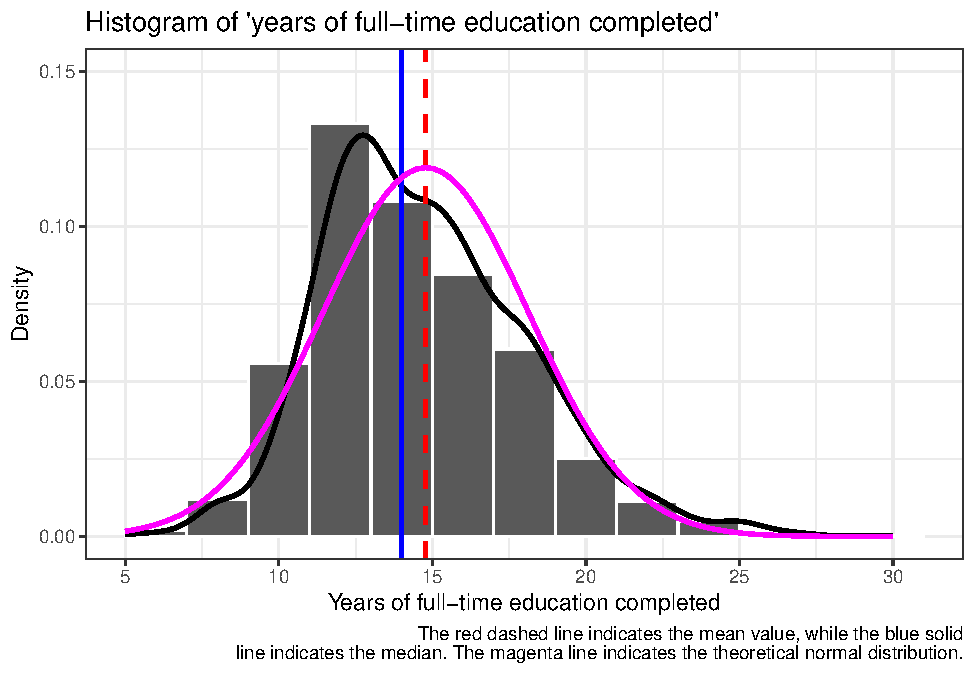
\includegraphics{AVCD-Assignment1-Edenhofer_files/figure-latex/distribution-eduyears-normal-1} \end{center}

\hypertarget{section-8}{%
\subsubsection{1.2}\label{section-8}}

\begin{Shaded}
\begin{Highlighting}[]
\NormalTok{ah21\_mod }\SpecialCharTok{\%\textgreater{}\%}
  \FunctionTok{ggplot}\NormalTok{(}\FunctionTok{aes}\NormalTok{(}\AttributeTok{x =}\NormalTok{ eduyrs, }\AttributeTok{fill =} \FunctionTok{factor}\NormalTok{(piketty\_dv))) }\SpecialCharTok{+}
  \FunctionTok{geom\_density}\NormalTok{(}\AttributeTok{alpha =} \FloatTok{0.4}\NormalTok{, }\AttributeTok{colour =} \StringTok{"gray"}\NormalTok{) }\SpecialCharTok{+}
  \FunctionTok{scale\_fill\_brewer}\NormalTok{(}\StringTok{""}\NormalTok{, }\AttributeTok{palette =} \StringTok{"Set1"}\NormalTok{, }\AttributeTok{direction =} \SpecialCharTok{{-}}\DecValTok{1}\NormalTok{, }
                      \AttributeTok{labels =} \FunctionTok{c}\NormalTok{(}\StringTok{"0"} \OtherTok{=} \StringTok{"Right"}\NormalTok{, }
                                 \StringTok{"1"} \OtherTok{=} \StringTok{"Left"}\NormalTok{)) }\SpecialCharTok{+}
  \FunctionTok{scale\_x\_continuous}\NormalTok{(}\StringTok{"Years of education"}\NormalTok{, }
                     \AttributeTok{breaks =} \FunctionTok{seq}\NormalTok{(}\DecValTok{5}\NormalTok{, }\DecValTok{30}\NormalTok{, }\DecValTok{5}\NormalTok{)) }\SpecialCharTok{+}
  \FunctionTok{scale\_y\_continuous}\NormalTok{(}\StringTok{"Density"}\NormalTok{, }
                     \AttributeTok{breaks =} \FunctionTok{seq}\NormalTok{(}\DecValTok{0}\NormalTok{, }\FloatTok{0.15}\NormalTok{, }\FloatTok{0.05}\NormalTok{)) }\SpecialCharTok{+}
  \FunctionTok{expand\_limits}\NormalTok{(}\AttributeTok{y =} \FloatTok{0.15}\NormalTok{) }\SpecialCharTok{+}
  \FunctionTok{labs}\NormalTok{(}\AttributeTok{title =} \StringTok{"Histogram of \textquotesingle{}years of full{-}time education completed\textquotesingle{} by left{-}right vote"}\NormalTok{) }\SpecialCharTok{+}
  \FunctionTok{theme\_bw}\NormalTok{() }\SpecialCharTok{+}
  \FunctionTok{theme}\NormalTok{(}\AttributeTok{legend.position =} \StringTok{"bottom"}\NormalTok{)}
\end{Highlighting}
\end{Shaded}

\begin{center}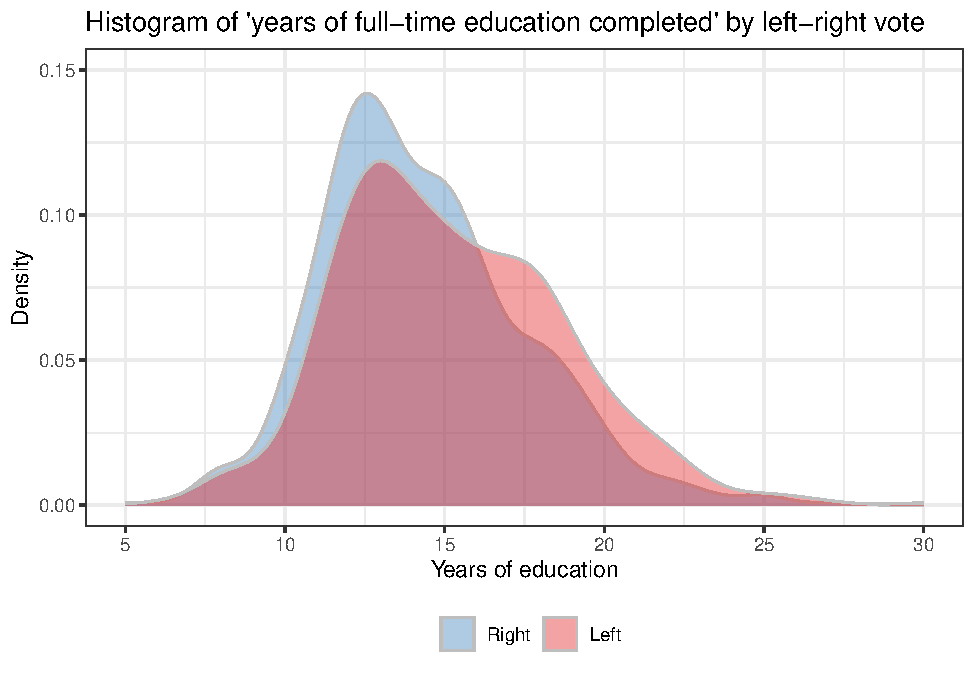
\includegraphics{AVCD-Assignment1-Edenhofer_files/figure-latex/edu-distribution-by-left-right-app-1} \end{center}

\hypertarget{section-9}{%
\subsubsection{1.3}\label{section-9}}

\begin{Shaded}
\begin{Highlighting}[]
\CommentTok{\# estimate logit}
\NormalTok{bi\_logit\_nl }\OtherTok{\textless{}{-}} \FunctionTok{glm}\NormalTok{(piketty\_dv }\SpecialCharTok{\textasciitilde{}}\NormalTok{ eduyrs }\SpecialCharTok{+} \FunctionTok{I}\NormalTok{(eduyrs}\SpecialCharTok{\^{}}\DecValTok{2}\NormalTok{), }
                \AttributeTok{family =} \FunctionTok{binomial}\NormalTok{(}\AttributeTok{link =} \StringTok{"logit"}\NormalTok{),}
                \AttributeTok{data =}\NormalTok{ ah21\_mod)}
\CommentTok{\# regression table}
\FunctionTok{modelsummary}\NormalTok{(bi\_logit\_nl,}
             \AttributeTok{estimate =} \StringTok{"\{estimate\}\{stars\}"}\NormalTok{, }
             \AttributeTok{coef\_map =} \FunctionTok{c}\NormalTok{(}\StringTok{"eduyrs"} \OtherTok{=} \StringTok{"Years of education"}\NormalTok{,}
                          \StringTok{"I(eduyrs\^{}2)"} \OtherTok{=} \StringTok{"Years of education squared"}\NormalTok{),}
             \AttributeTok{output =} \StringTok{"kableExtra"}\NormalTok{,}
             \AttributeTok{title =} \StringTok{"Logit model with non{-}linear education effect"}\NormalTok{) }\SpecialCharTok{\%\textgreater{}\%}
  \FunctionTok{kable\_styling}\NormalTok{(}\AttributeTok{latex\_options =} \StringTok{"hold\_position"}\NormalTok{)}
\end{Highlighting}
\end{Shaded}

\begin{table}[!h]

\caption{\label{tab:bi-logit-non-linear}Logit model with non-linear education effect}
\centering
\begin{tabular}[t]{lc}
\toprule
  & (1)\\
\midrule
Years of education & \num{0.020}\\
 & (\num{0.112})\\
Years of education squared & \num{0.002}\\
 & (\num{0.004})\\
\midrule
Num.Obs. & \num{1324}\\
AIC & \num{1812.1}\\
BIC & \num{1827.7}\\
Log.Lik. & \num{-903.067}\\
F & \num{11.790}\\
RMSE & \num{0.49}\\
\bottomrule
\end{tabular}
\end{table}

\hypertarget{exercise-2-1}{%
\subsection{Exercise 2}\label{exercise-2-1}}

\hypertarget{section-10}{%
\subsubsection{2.3}\label{section-10}}

\begin{Shaded}
\begin{Highlighting}[]
\CommentTok{\# models}
\NormalTok{multi\_logit }\OtherTok{\textless{}{-}} \FunctionTok{glm}\NormalTok{(piketty\_dv }\SpecialCharTok{\textasciitilde{}}\NormalTok{ eduyrs }\SpecialCharTok{+}\NormalTok{ gndr1 }\SpecialCharTok{+}\NormalTok{ blgetmg1 }\SpecialCharTok{+}\NormalTok{ ppltrst }\SpecialCharTok{+}\NormalTok{ gincdif, }
                   \AttributeTok{family =} \FunctionTok{binomial}\NormalTok{(}\AttributeTok{link =} \StringTok{"logit"}\NormalTok{),}
                   \AttributeTok{data =}\NormalTok{ ah21\_mod)}

\NormalTok{multi\_logit1 }\OtherTok{\textless{}{-}} \FunctionTok{glm}\NormalTok{(piketty\_dv }\SpecialCharTok{\textasciitilde{}}\NormalTok{ eduyrs }\SpecialCharTok{+}\NormalTok{ gndr1 }\SpecialCharTok{+}\NormalTok{ blgetmg1 }\SpecialCharTok{+}\NormalTok{ ppltrst }\SpecialCharTok{+} 
\NormalTok{                      gincdif }\SpecialCharTok{+}\NormalTok{ freehms }\SpecialCharTok{+}\NormalTok{ imwbcnt, }
                   \AttributeTok{family =} \FunctionTok{binomial}\NormalTok{(}\AttributeTok{link =} \StringTok{"logit"}\NormalTok{),}
                   \AttributeTok{data =}\NormalTok{ ah21\_mod)}

\CommentTok{\# regression table including both models}
\FunctionTok{modelsummary}\NormalTok{(}\FunctionTok{list}\NormalTok{(bi\_logit, multi\_logit, multi\_logit1),}
             \AttributeTok{estimate =} \StringTok{"\{estimate\}\{stars\}"}\NormalTok{, }
             \AttributeTok{coef\_map =} \FunctionTok{c}\NormalTok{(}\StringTok{"eduyrs"} \OtherTok{=} \StringTok{"Years of education"}\NormalTok{,}
                         \StringTok{"gndr1"} \OtherTok{=} \StringTok{"Gender dummy"}\NormalTok{,}
                         \StringTok{"blgetmg1"} \OtherTok{=} \StringTok{"Ethnic minority dummy"}\NormalTok{,}
                         \StringTok{"ppltrst"} \OtherTok{=} \StringTok{"Trust towards others"}\NormalTok{,}
                         \StringTok{"gincdif"} \OtherTok{=} \StringTok{"Attitudes towards redistribution"}\NormalTok{,}
                         \StringTok{"feehms"} \OtherTok{=} \StringTok{"LGBT+ people should be free to live as they wish"}\NormalTok{,}
                         \StringTok{"imwbcnt"} \OtherTok{=} \StringTok{"Immigrants make the country a worse/better place to live"}\NormalTok{),}
             \AttributeTok{output =} \StringTok{"kableExtra"}\NormalTok{, }
             \AttributeTok{title =} \StringTok{"Comparing bi{-} and multivariate logit models of voting for the left bloc"}\NormalTok{) }\SpecialCharTok{\%\textgreater{}\%}
  \FunctionTok{kable\_styling}\NormalTok{(}\AttributeTok{latex\_options =} \StringTok{"hold\_position"}\NormalTok{, }\AttributeTok{full\_width =}\NormalTok{ T) }\SpecialCharTok{\%\textgreater{}\%}
  \FunctionTok{add\_footnote}\NormalTok{(}\AttributeTok{label =} \StringTok{"See footnote 3 for interpreting the attiudinal covariates."}\NormalTok{, }\AttributeTok{notation =} \StringTok{"none"}\NormalTok{)}
\end{Highlighting}
\end{Shaded}

\begin{table}[!h]

\caption{\label{tab:multi-logit-red-table}Comparing bi- and multivariate logit models of voting for the left bloc}
\centering
\begin{tabu} to \linewidth {>{\raggedright}X>{\centering}X>{\centering}X>{\centering}X}
\toprule
  & (1) & (2) & (3)\\
\midrule
Years of education & \num{0.082}*** & \num{0.079}*** & \num{0.044}*\\
 & (\num{0.017}) & (\num{0.018}) & (\num{0.019})\\
Gender dummy &  & \num{0.080} & \num{0.162}\\
 &  & (\num{0.115}) & (\num{0.120})\\
Ethnic minority dummy &  & \num{0.518} & \num{0.707}*\\
 &  & (\num{0.321}) & (\num{0.347})\\
Trust towards others &  & \num{0.074}** & \num{0.008}\\
 &  & (\num{0.027}) & (\num{0.029})\\
Attitudes towards redistribution &  & \num{-0.401}*** & \num{-0.355}***\\
 &  & (\num{0.060}) & (\num{0.062})\\
Immigrants make the country a worse/better place to live &  &  & \num{0.201}***\\
 &  &  & (\num{0.030})\\
\midrule
Num.Obs. & \num{1324} & \num{1318} & \num{1305}\\
AIC & \num{1810.5} & \num{1753.0} & \num{1663.8}\\
BIC & \num{1820.8} & \num{1784.1} & \num{1705.2}\\
Log.Lik. & \num{-903.225} & \num{-870.515} & \num{-823.881}\\
F & \num{23.496} & \num{14.805} & \num{18.998}\\
RMSE & \num{0.49} & \num{0.48} & \num{0.47}\\
\bottomrule
\multicolumn{4}{l}{\textsuperscript{} See footnote 3 for interpreting the attiudinal covariates.}\\
\end{tabu}
\end{table}

\FloatBarrier

\hypertarget{references}{%
\section*{References}\label{references}}
\addcontentsline{toc}{section}{References}

\hypertarget{refs}{}
\begin{CSLReferences}{1}{0}
\leavevmode\vadjust pre{\hypertarget{ref-abou-chadi_brahmin_2021}{}}%
Abou-Chadi, Tarik, and Simon Hix. 2021. {``Brahmin {Left} Versus
{Merchant} {Right}? {Education}, Class, Multiparty Competition, and
Redistribution in {Western} {Europe}.''} \emph{The British Journal of
Sociology} 72 (1): 79--92.
\url{https://doi.org/10.1111/1468-4446.12834}.

\leavevmode\vadjust pre{\hypertarget{ref-becker2009human}{}}%
Becker, Gary S. 2009. \emph{Human Capital: A Theoretical and Empirical
Analysis, with Special Reference to Education}. Chicago: University of
Chicago Press.

\leavevmode\vadjust pre{\hypertarget{ref-cavaille2019education}{}}%
Cavaille, Charlotte, and John Marshall. 2019. {``Education and
Anti-Immigration Attitudes: Evidence from Compulsory Schooling Reforms
Across Western Europe.''} \emph{American Political Science Review} 113
(1): 254--63.

\leavevmode\vadjust pre{\hypertarget{ref-chiaramonte2019towards}{}}%
Chiaramonte, Alessandro, and Vincenzo Emanuele. 2019. {``Towards
Turbulent Times: Measuring and Explaining Party System (de-)
Institutionalization in Western Europe (1945--2015).''} \emph{Italian
Political Science Review/Rivista Italiana Di Scienza Politica} 49 (1):
1--23.

\leavevmode\vadjust pre{\hypertarget{ref-gailmard_statistical_2014}{}}%
Gailmard, Sean. 2014. \emph{Statistical {Modeling} and {Inference} for
{Social} {Science}}. Cambridge: Cambridge University Press.

\leavevmode\vadjust pre{\hypertarget{ref-putnam2000bowling}{}}%
Putnam, Robert D. 2000. \emph{Bowling Alone: The Collapse and Revival of
American Community}. New York: Simon; schuster.

\leavevmode\vadjust pre{\hypertarget{ref-yang2022more}{}}%
Yang, Songtao. 2022. {``More Education, Less Prejudice Against Sexual
Minorities? Evidence from Compulsory Schooling Reforms.''} \emph{Applied
Economics Letters} 29 (19): 1840--46.

\end{CSLReferences}

\end{document}
